\chapter{From the Moscow Circle to the Prague School and Trubetzkoy's \emph{Grundzüge}}
\label{ch.prague}

Work in phonology continued among {\Baudouin}'s students such as Lev
{\Ščerba} and \name{Yevgeny}{Polivanov} (1891--1938) in St. Petersburg, but in the
years immediately preceding the {Russian} revolution an approach to the
study of language developed in Moscow which was largely (though not
entirely) independent of {\Baudouin}'s views.\footnote{For discussion of
  the history and development of the St. Petersburg/Leningrad and
  Moscow schools of linguistics in the early 20th century, see
  \citealt{iosad21:soviet.phonology}. Although of considerable
  interest in themselves, the works of these scholars are somewhat
  orthogonal to the present work, and cannot be considered adequately
  here.} An interest in problems of poetics, literary analysis, and
general artistic structure was combined with the influence of Slavic
and historical linguistics in the discussions of a group of younger
scholars, who were encouraged to develop this wide range of problems
on the basis of the novel ideas they found in the works of {\Saussure}
and {\Baudouin}. The result was an independent perspective on the basic
issues in language and linguistics, much different from the rather
phonetically oriented views of the St. Petersburg/Leningrad school.

The turbulence of the revolution and the period immediately following
broke up this group, forcing many of them to emigrate. During the
1920s, however, several of the most important figures found themselves
in or near Prague, where their collaboration was reconstituted and
expanded around the activities of the {Linguistic Circle of Prague},
organized by the {Czech} linguist and literary historian \name{Vilém}{Mathesius}
(1882–1945). Besides their actual research, this group was
particularly vigorous in presenting its point of view to the larger
world of linguistics and in aggressively recruiting other scholars to
the novelties of structuralist phonology. This crusading spirit may
have contributed as much as did the actual results of their work to
the Prague school linguists' success in essentially changing the
character of European linguistics. Novelty and excitement, especially
when combined with the activity of such powerful intellectual figures
as {\Jakobson} and {\Trubetzkoy}, are often irresistible, as linguistics has
seen in other contexts since.

It is interesting to note that the work usually identified as the
virtual codification of Prague school phonology, {\Trubetzkoy}'s
\textsl{Grundzüge der Phonologie}
(\citealt{trubetzkoy39:grundzuge}\footnote{Citations from the
  \textsl{Grundzüge} in the present work are generally the author's
  translations based on the 1957 {French} edition by J. Cantineau.}), was
written by one who was not closely identified with the program of the
earlier Moscow Circle, and who worked in Vienna rather than in
Prague. Certainly other prominent members of the Prague Circle had
other interests, and a full treatment of their views would have to go
well beyond the discussion here centering on {\Trubetzkoy}. Nonetheless,
it is difficult to dispute the claim that in terms both of his
centrality in discussions on specifically phonological issues and of
his influence on later scholarship, {\Trubetzkoy} represents the essence
of `Praguian' phonology. His intimate collaboration with {\Jakobson} in
the context of the Prague Circle, together with his role as perhaps
its most prominent representative to the international community (both
at the time and in the subsequent literature), makes his work the
fundamental and most important statement of its views.

\section{The background of the Prague Circle and the life of Trubetzkoy}
\label{sec:backgr-prag-circle}

The Moscow Linguistic Circle was founded in 1915 by a group of seven
young {Russian} linguists, ``having as its aim the study of linguistics,
poetics, metrics and folklore'' as stated in its authorization
\citep[530]{jakobson65:terms}. Central among these was Roman
{\Jakobson}, who was the president of the circle from 1915 to 1920; he
and other members such as N. F. Jakovlev\ia{Jakovlev, Nikolai} (a specialist in Caucasian
languages) were noted for their contributions to more or less `pure'
linguistics, but from the beginning this group gave a very prominent
place to what we would now consider interdisciplinary perspectives
drawn from the study of art and literature, and especially of poetry.

{\Jakobson} himself (born in 1896 in Moscow) was primarily interested in
the study of poetry, and initially intended to specialize in literary
history. In addition to the Linguistic Circle, he was also a member of
several other innovative literary and poetic circles both in Moscow
and in St. Petersburg. He was rather caught up in the general early
twentieth-century interest in the analytical study of formal structure
in art, architecture, music, and verse, but came early to the
conclusion that the study of form in poetry could only proceed on the
basis of an insight into the structure of language. His early work was
dominated by poetic considerations, and while this interest continued
to be central throughout his life, his linguistic studies gradually
led him to an involvement not only in questions of folklore, Slavic
and \ili{Indo-European} metrics, etc., but also in Slavic historical
linguistics (the dominant concern of the linguistics faculty in
Moscow) and eventually in general linguistics.

\begin{wrapfigure}{l}{.35\textwidth}
  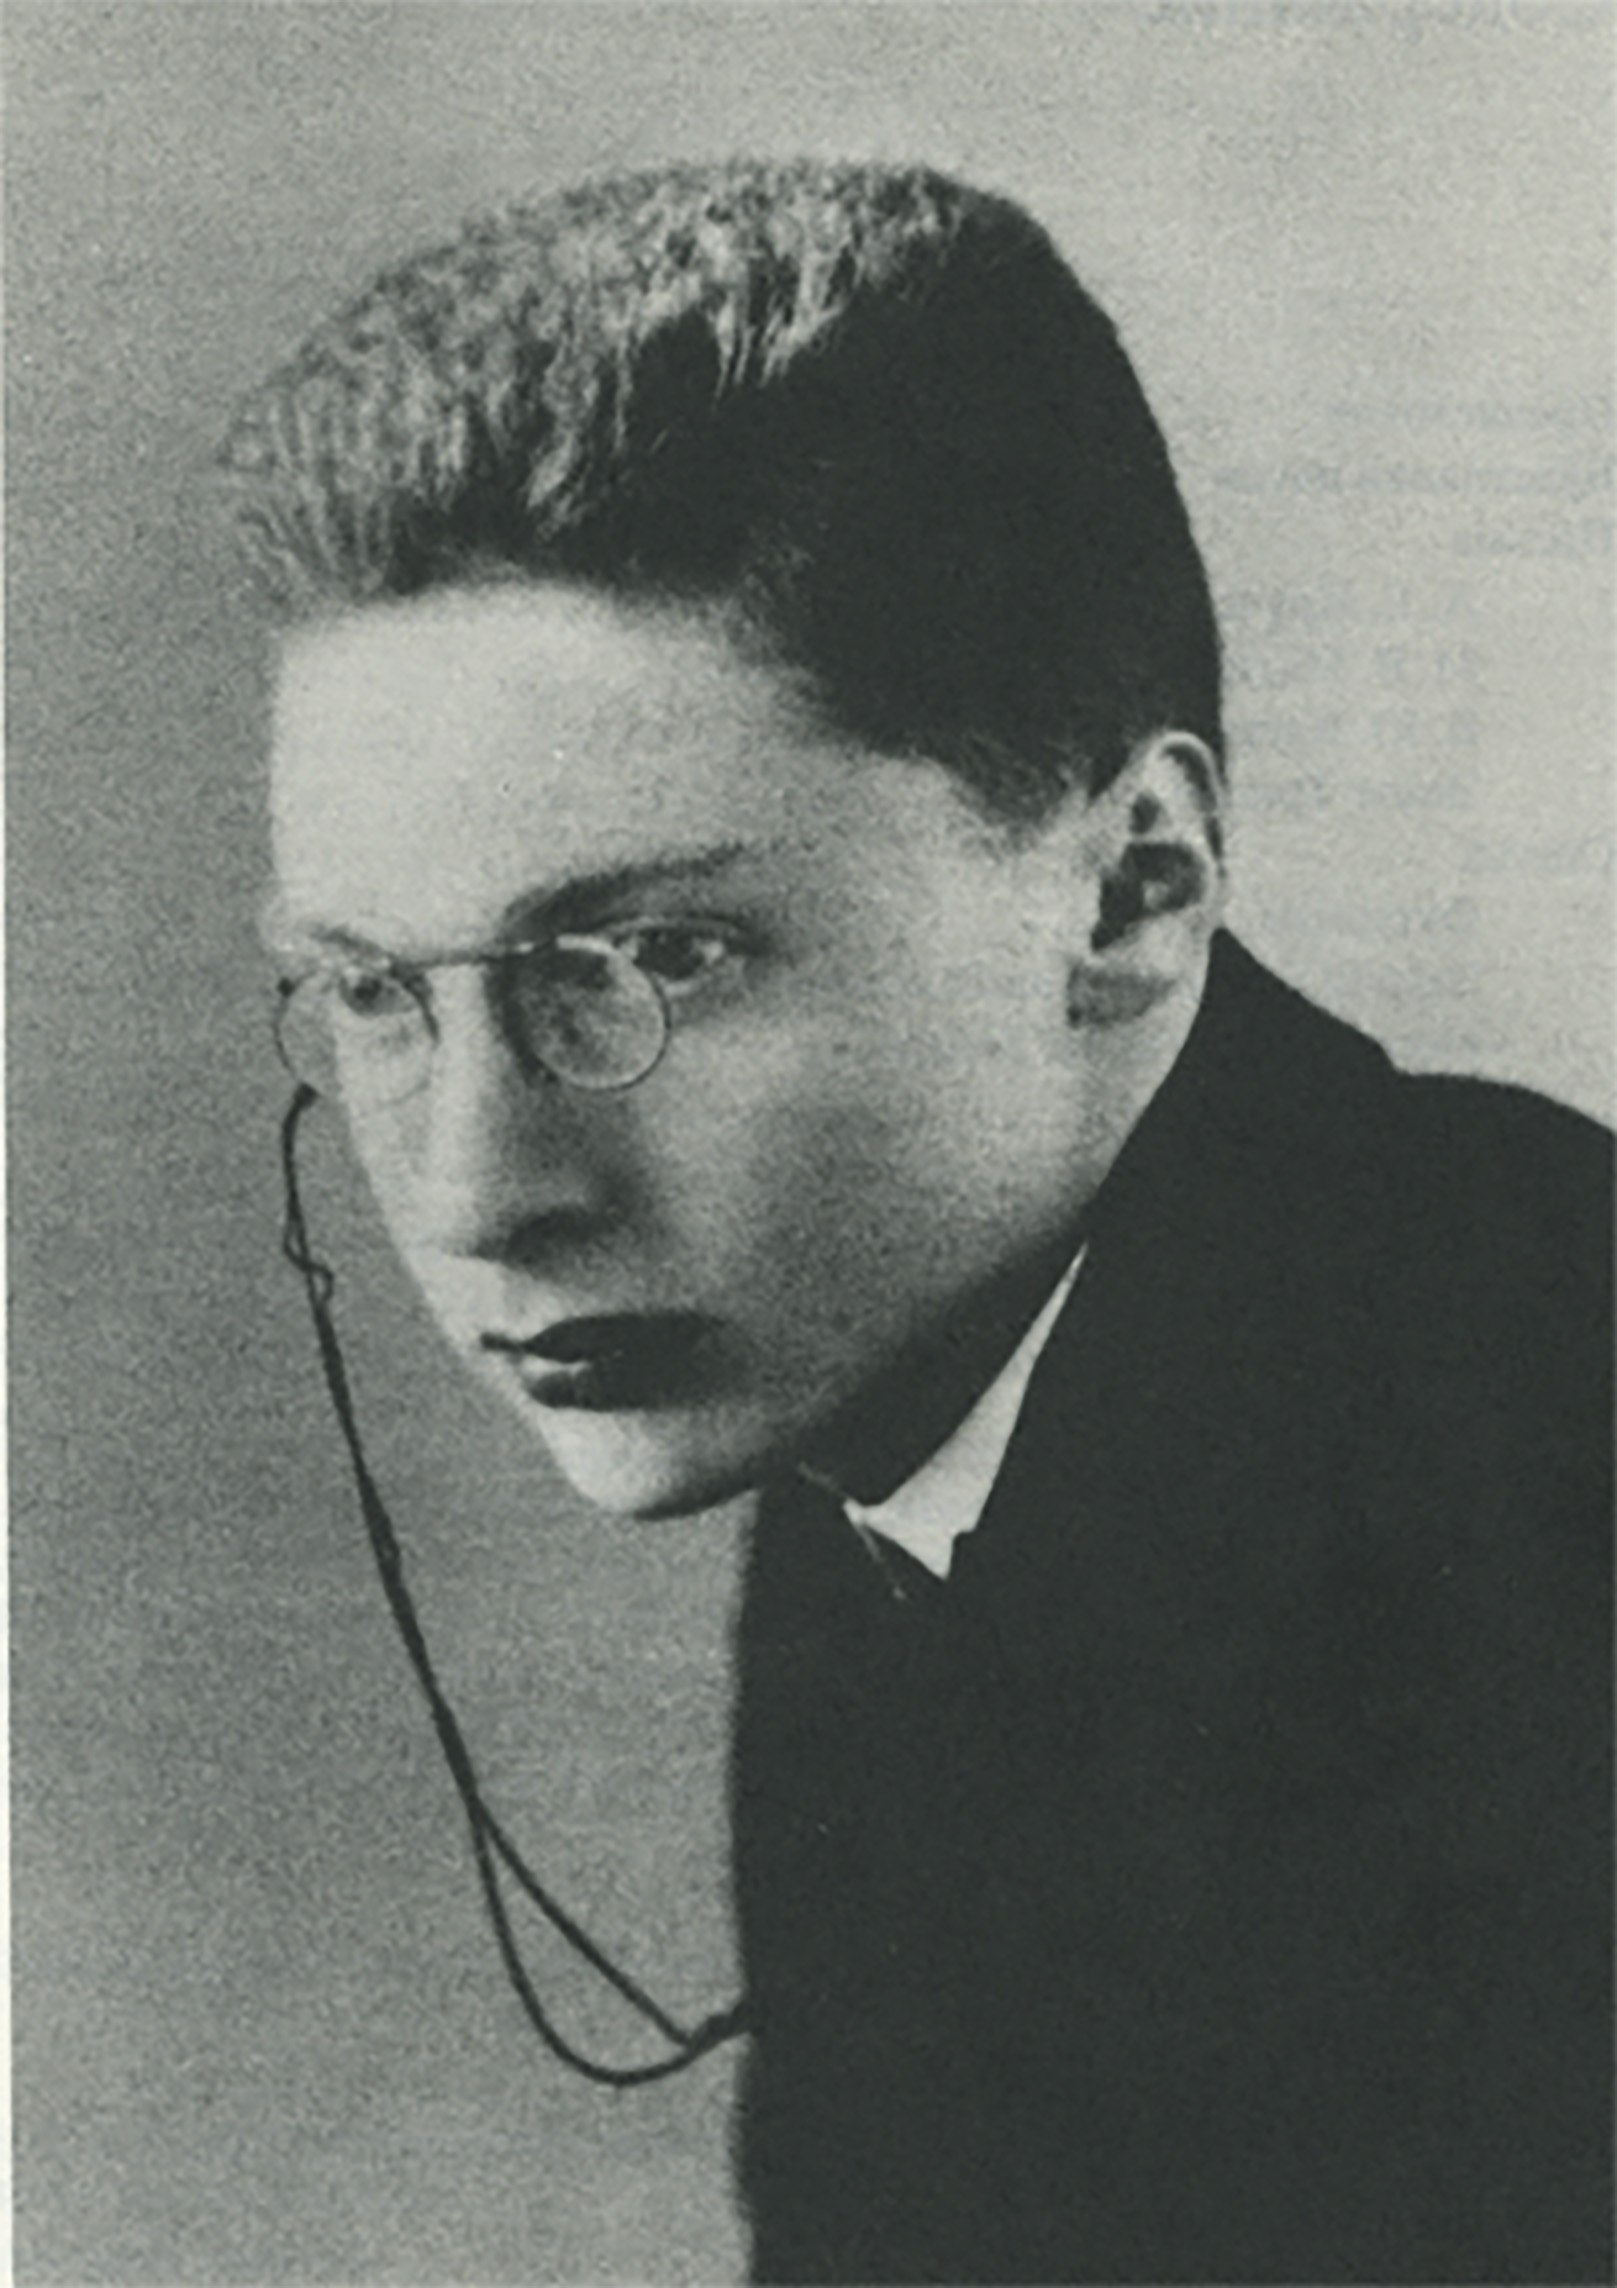
\includegraphics[width=.9\textwidth]{figures/RomanJakobson-1916.jpg}
  \caption{Roman Jakobson in 1916}
  \label{fig:ch.prague_jakobson_1916}
\end{wrapfigure}
\citet[631]{jakobson62:retrospect} notes that when he submitted a
list of proposed readings to his adviser, the only item that was not
approved as a part of his program was {\Ščerba}'s monograph on \ili{Russian}
vowels \citep{shcherba12:russian.vowels}; and that, naturally, it was
just this work with its background in {\DeCourtenay}'s (late)
views on the nature of phonological structure and the \isi{phoneme} that he
read first. The notion of a unit of \isi{sound structure} which represented
exactly the aspects of the phonetic material that could serve to
differentiate words from one another seemed the natural basis for an
analysis which would extend to literature (and especially to verse)
the study of formal relationships as in other arts.

{\Baudouin}'s work thus came to have an indirect influence on the early
discussions of the Moscow Linguistic Circle, and another of its
members soon introduced the views of {\Saussure}. \name{Sergej}{Karcevskij}
(1884--1955) had emigrated to Geneva in 1907, where he studied
linguistics with {\Saussure}, {\Bally}, and {\Sechehaye}. In 1917 he returned
to Moscow, where he became a member of the Linguistic Circle and
presented the views of {\Saussure}'s \textsl{Cours} (just published) to
his {Russian} colleagues. After leaving Moscow again in 1919, he spent
additional time with {\Meillet} (in 1920-22) and was awarded a doctorate
in 1927 from Geneva, where he later taught. In his contributions both
to the Moscow Circle and, later, in Prague, {\Karcevskij} facilitated a
familiarity on the part of both groups with the `Geneva school' view
of language.

By the beginning of the twentieth century, the notion of a kružok or
'circle' had a rather long history among {Russian} intellectuals
\citep{jakobson65:terms}. These small, semi­formal societies were
generally composed of young adherents of some more or less avant-garde
view, who met in one another's homes for discussion. Since such groups
(nominally devoted to literary concerns or the like) were also a
source of much clandestine political activity, they unfortunately
tended to arouse the interest of the tsarist police. In order to
establish its own bona fides and thus avoid this consequence, the
\emph{Moskovskij lingvestičeskij kružok} operated under the auspices
of the Moscow Dialectological Commission, associated with the {Russian}
Academy of Sciences. The Dialectological Commission, itself founded in
1904 to provide a forum for young scholars interested in the study of
\ili{Russian}, was at the time the most active group engaged in linguistic
and folkloristic research. Among its more active members was the
Prince \name{Nikolaj Sergeevič}{Trubetzkoy}, with whom {\Jakobson} and the Moscow
Circle linguists thus came into contact.

{\Trubetzkoy} was born in Moscow in 1890. His father, Prince Sergej
Trubetzkoy, was a professor of philosophy at the University of Moscow
and, at the time of his death in 1905, rector of the
university. Evidently rather precocious, the young {\Trubetzkoy} had
begun to study the ethnology and \isi{ethnography} of the Finno-Ugric
peoples of Russia at the age of thirteen; and at the age of fifteen,
he published two articles on the folklore of the Finns and that of the
Voguls, Ostyaks, and Votyaks. Still in his teens, he also worked on
the languages of the Paleo-Siberian group, sketching a grammar of
Kamchadal and doing comparative work on this language and Chukchee. It
is reported that \name{Vladimir}{Bogoraz}, the most eminent specialist in Chukchee
and Koryak at the time, was quite upset when he discovered that the
promising scholar with whom he had been in correspondence for some
time was in fact still of high school age.

When he entered the university in 1908, {\Trubetzkoy} wanted to
specialize in ethnology and \isi{ethnography}, but the faculty within which
these subjects were taught in Moscow treated them as disciplines of
the natural rather than the social and human sciences, as {\Trubetzkoy}
would have preferred. He thus began to study in the department of
philosophy and psychology, but soon discovered that it was impossible
to pursue his main interests within this program either. As a result,
he transferred in his second year to the department of
linguistics. Here too his studies were not concentrated on his primary
area of interest, since the required program was mostly devoted to
\ili{Indo-European} historical and comparative grammar, but he decided to
continue for primarily methodological reasons. Linguistics seemed to
him to be based on more rigorous grounds than any other branch of the
human sciences, and \ili{Indo-European} studies were obviously much better
developed than any other branch of the field and thus the best place
to learn its methods.

Ih 1911 {\Trubetzkoy} spent his summer vacation in the Caucasus with
Professor \name{Vsevolod}{Miller}, president of the Moscow Ethnographic Society and
a specialist in Ossetic. On this trip he began work on the languages
of the Northwest Caucasian family; and, indeed, for the rest of his
life he would devote a considerable share of his scholarly attention
to these languages as well as those of the Northeast Caucasian
group. In 1913 he presented his thesis in linguistics, dealing with the
range of expression of the future in \ili{Indo-European}, and was accepted
into the faculty of the department. After spending 1913-14 in {Leipzig}
studying with {\Brugmann}, {\Leskien}, and others (and where he came into
contact with \name{Leonard}{Bloomfield}, who was there at the same time), he
prepared for his doctoral examinations and gave the required two
public lectures to qualify for the doctorate, after which he was made
the equivalent of an assistant professor. He began by teaching
{Sanskrit}, and intended to add Avestan and Old Persian the following
year, but by 1916 his attention was drawn irresistibly to questions of
methodology and to historical Slavic phonology.

The linguistics faculty in Moscow at this time was completely
dominated by the views of F. F. {\Fortunatov} (1848-1914), who had
developed an essentially Neo\-grammarian position on historical
reconstruction in a particularly formal and rigorous way. In
\citeyear{shakhmatov15:common.slavic}, Alexei {\Šaxmatov} (1864--1920)
published a comprehensive reconstruction within this tradition of the
history of \ili{Russian} and of common \isi{Slavic}, a work which {\Trubetzkoy} felt
exemplified perfectly all of the faults in {\Fortunatov}'s
methodology. He presented a highly criticial analysis of {\Šaxmatov}'s
work at the Moscow Dialectological Commission, which created a
furor. As a result of this confrontation, he decided to devote his
efforts to substantiating his position in detail, and intended to
write his own \textsl{Prehistory of Slavic}. This project became
something of an obsession with him over a number of years, and most of
his attention was for a time concentrated on studies related to it.

\begin{wrapfigure}[17]{r}{.35\textwidth}
  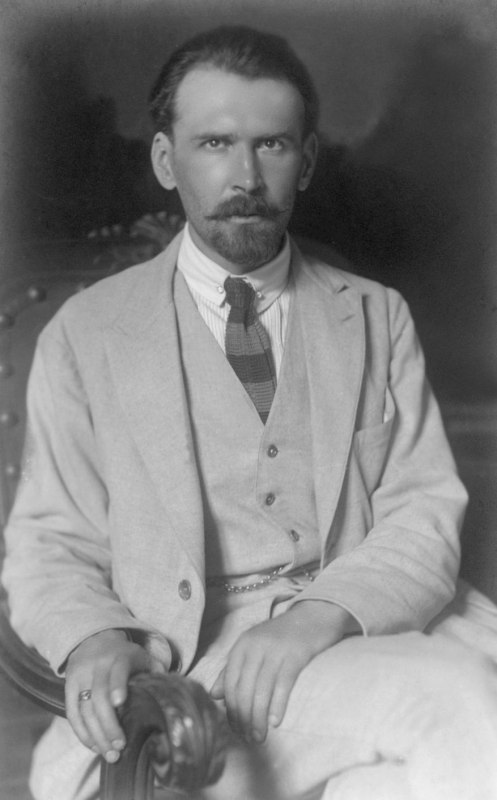
\includegraphics[width=.9\textwidth]{figures/Trubetzkoy_younger.jpg}
  \caption{Prince Nikolai Sergeievič Trubetzkoy (1927)}
  \label{fig:ch.prague_trubetzkoy_younger}
\end{wrapfigure}
In the turmoil of 1917, Prince {\Trubetzkoy} was forced to flee
Moscow. Escaping through the Caucasus (where an independent republic
existed briefly in the period immediately after the October
revolution), he found a temporary refuge in Rostov, but soon had to be
evacuated again. In the process, nearly all of his notes and
manuscripts were lost, including drafts of parts of the
\textsl{Prehistory}. During 1920-22, he occupied a position in Slavic
philology and comparative linguistics at the University of Sofia in
Bulgaria, but as political conditions once more became difficult for
him there, he was forced to move again. Hoping to find a position in
newly independent Czechoslovakia, he settled ``temporarily'' in Vienna,
where he was offered a chair in Slavic philology. In fact, he occupied
this position for the rest of his life.

In the meantime, {\Jakobson} too left Russia and took up his studies in
Prague in 1920. He contacted {\Trubetzkoy} at this time in Sofia, and an
extensive series of letters between the two began at this time. Their
contents (published as \citealt{jakobson75:trubetzkoy.letters}),
continuing up to {\Trubetzkoy}'s death, provide valuable insights into
the. development of the notion of 'phonology' during this period as
well as their authors' attitudes toward their own work and that of
others.

In this period, {\Trubetzkoy} was primarily interested in Slavic
historical ques\-tions related to his Prehistory, and the early
correspondence with {\Jakobson} is dominated by such issues. {\Jakobson}
himself was largely occupied with questions of poetics and metrics, as
illustrated in his first major work, \textsl{On {Czech} Verse}
\citep{jakobson23:o.cesskom.stixe}; but as a natural development of
this along lines suggested already in discussions of the Moscow
Circle, he was increasingly interested in the more general notion of
\isi{sound structure} in language. His attempts to interest {\Trubetzkoy} in
the development of the theoretical study of phonemic patterns received
little more than polite response at first; but in 1926, {\Jakobson} found
the key to {\Trubetzkoy}'s attention.

In a long letter outlining the significance of phonological studies
for \isi{historical change}, he suggested that a genuinely explanatory and
predictive theory in this area could be supplied by a consideration of
changes as taking place not blindly and fortuitously in sounds but,
rather, functionally in phonological systems. The interpretation of
\isi{sound change} as motivated by the structure of such systems could thus
replace what {\Jakobson} saw as unsatisfactory in the Neogrammarian and
Saussurian views; but obviously it was necessary first to have a clear
idea of what such systems were like and of the laws governing their
structure.

{\Trubetzkoy} was immediately persuaded that in such a direction lay
answers to the questions of methodology in historical linguistics that
had preoccupied him for so long, and from then on the direction of his
work changed radically. Though he continued to teach and to do
research on historical Slavic matters, his primary interest became the
study of \isi{regularities} in synchronic phonological systems. He soon saw
that his earlier plan for his \textsl{Prehistory} would have to be totally
rethought from the new point of view; and, indeed, in the face of his
new goals, the \textsl{Prehistory} rapidly disappeared from view. Instead, he
concentrated his attention on studying the phonological systems of as
many languages as he could find adequate descriptions of, in order to
uncover in this inductive fashion the basic \isi{regularities} governing
phonological patterns.

The cooperation between {\Trubetzkoy} and {\Jakobson} was further enhanced,
and given an organizational vehicle, by the founding of the Linguistic
Circle of Prague.\footnote{\citet{Toman95:prague} provides a rich and
  detailed description of the background, life, and times of the
  Prague Circle.} The {Czech} professor \name{Vilém}{Mathesius} had admired the
atmosphere and work of the Moscow Linguistic Circle, and in 1925
explored the idea of starting a similar group in Prague with his
student B. Trnka\ia{Trnka, Bohumil}, {\Jakobson}, and {\Karcevskij} (who was also in Prague at
this time). In October of the following year, the \emph{Prazsky
  linguistick{\'y} krou{\"z}ek} held its first meeting, and the group
rapidly attracted a number of {Czech} (and other) linguists to its
discussions as well as {\Trubetzkoy} from nearby Vienna. As with its
predecessor in Moscow, the Prague Circle involved literary and
philosophical figures as well as linguists: Husserl\ia{Husserl, Edmund} and Carnap\ia{Carnap, Rudolf}, for
example, as well as several novelists and poets addressed its
sessions. Nonetheless, its primary activity (at least as far as it
affected the outside world) was the development of a `structuralist'
perspective on language, and particularly on phonology.

In the manner of artistic and literary movements of the time, this
development found early expression in manifestos presented to
international gatherings. It must be recognized that despite the
earlier work of {\Saussure}, {\Baudouin}, and their followers, the character
of linguistic research still had not fundamentally changed. The field
was dominated by historical studies of the atomistic, Neogrammarian
sort on the one hand, and by detailed observational phonetic studies
on the other. The notion of a language as a system of related elements
(rather than a more or less disjointed collection of independent ones)
had as yet had little impact on the methodological premises of
linguistic investigations. Similarly, the notion that a linguistically
{significant} description of the sound system of a given language should
explicate the ways in which distinct forms are differentiated from one
another, rather than providing a uniformly fine-grained account of the
acoustic and/or articulatory events associated with the production of
particular words, had still not effectively emancipated phonetic
studies from the obsession with masses of detail in which they were
effectively mired as instrumental techniques of observation were
refined. 

The phonologists of the Prague school thus felt they were leading a
sort of crusade against entrenched fundamental misconceptions, and
they adopted an aggressive, sometimes confrontational approach in the
effort to put across their ideas. As often happens in such
circumstances, the very feeling of novelty and lively activity
generated by the `phonological movement' proved irresistible to many,
especially younger scholars. {\Trubetzkoy} himself, as indicated in his
letters to {\Jakobson}, saw in an almost Manichaean fashion a field
divided between those who were ``with us'' and those who were not. The
ranks of the former swelled significantly with each passing
international gathering. 

The work of the Prague Circle focused immediately on preparations for
the upcoming {First International Congress of Linguists}, to be held in
The Hague in 1928. For this meeting, a set of general questions about
the nature of the field and its methods had been formulated by the
organizers, and participants were invited to prepare propositions
addressing these issues. In response to the question ``Quelles sont les
méthodes les mieux appropriées a un exposé complet et pratique de la
grammaire d'une {langue} quelquonque?'' \citet{jakobson28:first.icl}
prepared a set of propositions outlining and arguing for the basic
goals of phonology. Intended to address the perceived failures both of
neogrammarian historical linguistics and of phonetics, these
propositions (which were signed also by {\Trubetzkoy} and {\Karcevskij})
advocated a fundamental {change} of direction in linguistic
research. While obviously controversial, they were in fact
enthusiastically approved by many participants at the Congress,
encouraging their formulators to further efforts (assuming this was
needed).

According to {\Jakobson}'s proposals, the tasks of phonology are (a) to
identify the characteristics of particular phonological systems, in
terms of the language-particular range of significant differences
among ``acoustico-motor images''; (b) to specify the types of such
differences that can be found in general, and in particular to
identify `\isi{correlations}', or recurrent differences that serve to
characterize multiple pairs of elements (as e.g. \isi{voicing} separates
\emph{p} from \emph{b}, \emph{t} from \emph{d}, etc.); (c) to
formulate general laws governing the relations of these \isi{correlations}
to one another within particular phonological systems; (d) to account
for \isi{historical change} in terms of the \isi{phonological system} (rather than
the individual sound) which undergoes it, and especially to construe
such changes as teleologically governed by considerations of the
system; and, finally, (e) to found phonetic studies on an acoustic
rather than an articulatory basis, since it is the production of sound
that is the goal of linguistic phonetic events and that gives them
their social character. In this program, there was undoubtedly
something to offend just about anyone who accepted the then-current
assumptions of the field.

While {\Jakobson}'s propositions diverged from the practice of other
linguists in all of their major respects, this was especially true in
his urging a concentration on the system of distinctive sound
differences to the exclusion of other phonetic facts, and in proposing
a teleological, system-determined conception of \isi{linguistic change}. It
is by no means clear that the latter notion ever really prevailed:
while historical studies came soon to be cast in terms of changes
undergone by the \isi{phonological system}, the role played by the system in
motivating change generally in a teleological fashion was stressed
more by theoreticians (e.g. \citealt{martinet55:economie}; see
chapter~\ref{ch.martinet}) than by the mainstream of practicing
historical linguists (which is not to deny that {\Martinet} himself did
substantive work of a historical nature).

In descriptive studies, on the other hand, the eventual victory of the
`phonological' perspective was virtually complete. Its essential
insight was basically no different from {\Saussure}'s: in order to study
the sound system of a particular language, it is necessary to focus on
the ways in which sound differences do or do not differentiate
distinct forms within that language. The fact that {\Jakobson} posed this
basic principle in an explicit and persuasive way, at a time when the
field was prepared to recognize the deficiencies of the alternatives
to it, led to its acceptance. Though this did not take place
overnight, the dominance of purely phonetic and historical studies
gave way before long to analyses concentrating on the distinctive
function of sound elements.

It is necessary to recognize that the specific way in which the Prague
linguists intended to carry out this study (to wit, by establishing
systems of elements composed of exactly the distinctive properties of
phonetic entities) is not the only way it could be pursued. Recall the
discussion above in chapter~\ref{ch.saussure_sound} concerning
different conceptions of phonemic representation, and different ways
of carrying out the essential aspects of {\Saussure}'s
program. Nonetheless, many linguists accepted the notion that studying
exclusively the distinctive elements (or `phonemes' in one specific
sense) was a necessary concomitant of abandoning a naive phonetic
approach to language—in part, probably, for the simple reason that it
was in this concrete form that the basic insight of phonology was
presented to them.

After the Hague congress, the Prague Circle immediately began
preparations for an {International Congress of Slavists} to be held in
Prague in 1929. Again at this meeting, a set of `theses' was
formulated in the name of the Prague Circle
\citep{theses29:prague.slavic}, circulated at the congress, and
discussed. These theses extended and refined the lines suggested by
{\Jakobson} at The Hague, and again resulted in both controversy and
conversions. Indeed, it appears (according to
\citealt{jakobson65:terms}) that the controversy engendered by the
circle's theses was sufficiently ardent that the proceedings of the
plenary sessions (at which their point of view was the most prominent)
were mysteriously `lost', and this volume of the congress's
\textsl{Transactions} was never published.

During the 1930s the growth and international prominence of phonology
and the Praguian approach to it was prodigious, though this was more a
matter of individual scholars than of whole institutions. Academic
employment was anything but abundant, and the onset of the depression
hardly improved this. {\Jakobson} was only offered a {regular} faculty
position (as professor in Brno) in 1931, and then a combination of
economic difficulties and academic political opposition had the result
that he was not officially nominated until 1933. Even then, he was not
confirmed (and thus received no salary) until the following
year. {\Trubetzkoy} had a secure position in Vienna, but most of his
teaching was committed to Slavic rather than to general linguistics or
phonology \emph{per se}.

\begin{wrapfigure}{r}{.4\textwidth}
  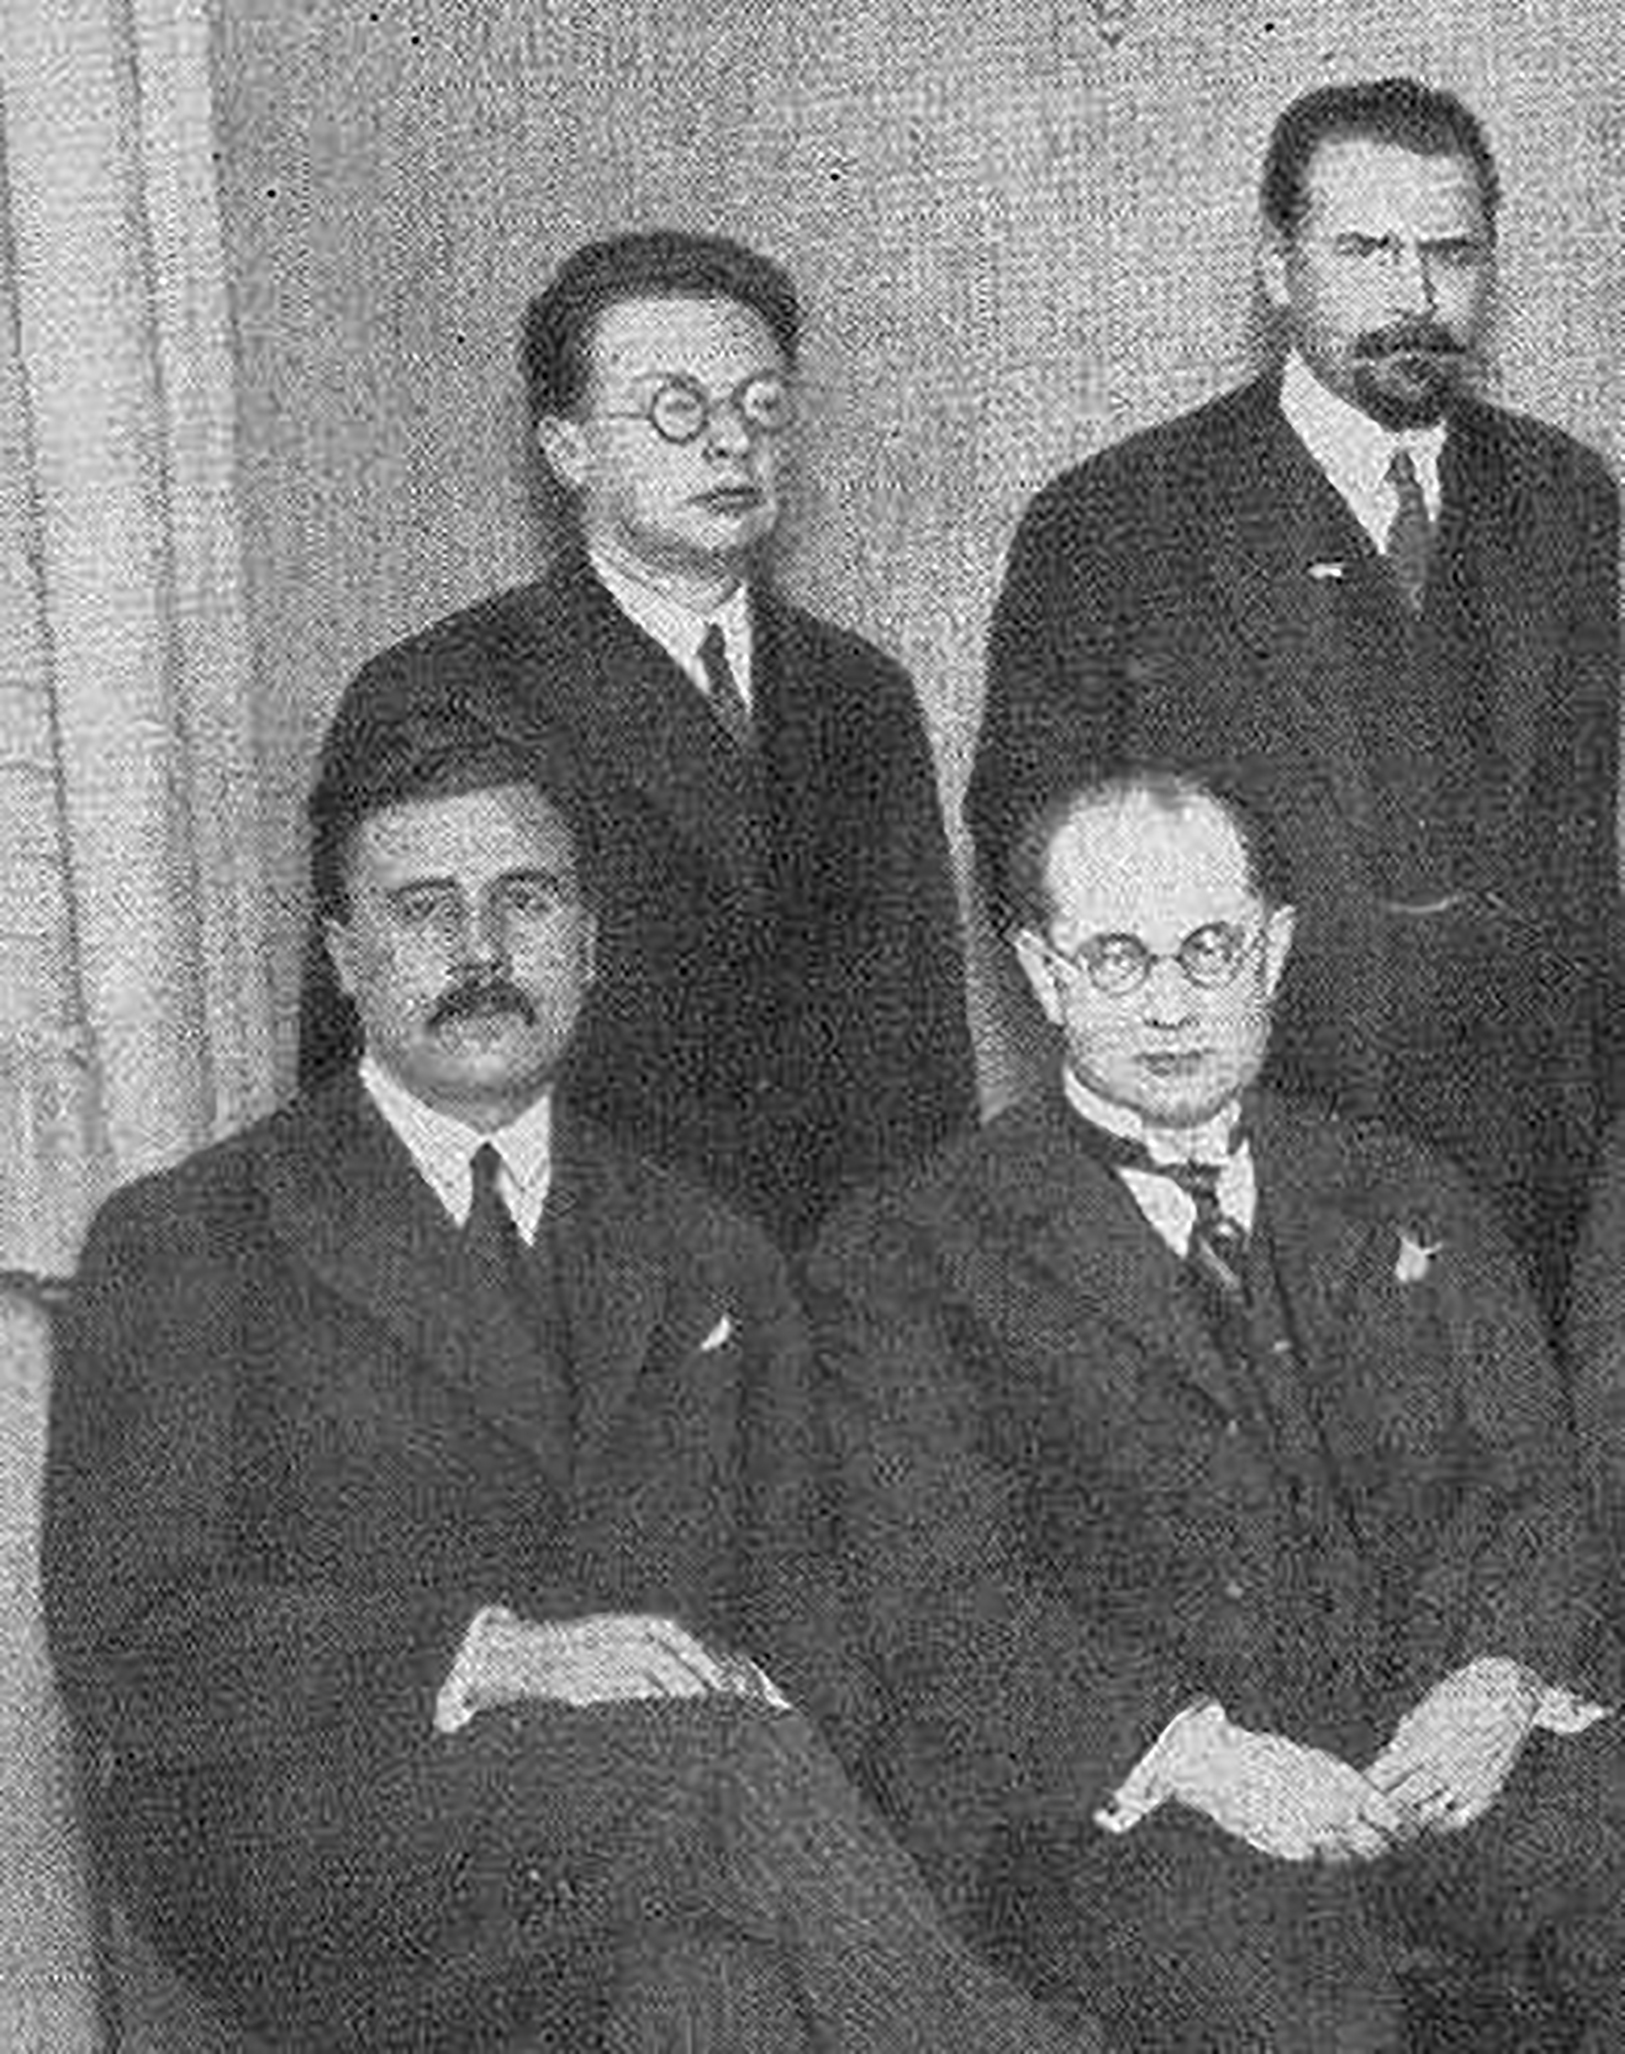
\includegraphics[width=.9\textwidth]{figures/PragueCircle1930.jpg}
  \caption{Detail from the 1930 International Phonology Meeting\\
    (Standing: Jakobson, Trubetzkoy; Sitting: V. Doroshevsky (Polish
    Slavist, a student of Baudouin de Courtenay in Kazan),
    V. Mathesius)}
  \label{fig:ch.prague_trubetzkoy_prague_circle}
\end{wrapfigure}
Both {\Jakobson} and {\Trubetzkoy} were none\-the\-less in contact with most of the
important figures in the field, as well as a significant number of the
less prominent ones. Some of the former, such as {\Sapir}, {\Meillet}, and
\name{Joseph}{Vendryès}, proved receptive in varying degrees to their ideas, and
these consequently became more widely known. In Prague itself, the
Linguistic Circle initiated a series of \textsl{Travaux du cercle
  linguistique de Prague} with a set of studies prepared for the
Slavistic Congress in 1929, and these became the primary forum for
discussion of Praguian phonology. Following on their successes at the
congresses of the preceding years, the Prague linguists organized an
International Phonology Meeting in 1930, which was attended by
scholars from a number of countries. In 1932, an International
Phonological Association was established in connection with the
International Permanent Committee of Linguists (CIPL), the body
responsible for organizing the international congresses of
linguistics. This association distributed copies of {\Trubetzkoy}'s
\textsl{Anleitung zu phonologischen Beschreibungen}
\citep{trubetzkoy68:principles} to its members in many countries.

Dedicated attention to matters of organization and `public relations',
as well as intellectual ones, together with a {nucleus} of ardent
supporters, thus secured a central place for Praguian views in the
development of linguistics in the 1930s. This development was greatly
complicated, however, by the economic difficulties and political
crises which upset both communication and the careers of many
individual linguists.

{\Trubetzkoy} began work on a comprehensive synopsis of the central
notions of phonology, incorporating analyses of numerous languages as
well as the theoretical principles underlying phonological
theory. Increasingly affected by a heart ailment, he was particularly
eager to see this project completed. In 1938 (perhaps partly as a
result of an especially unpleasant Gestapo raid on his apartment, when
many of his papers were destroyed or confiscated), he suffered a final
attack and died on 25 June. He managed to complete a draft of the
first (and principal) volume of his introduction just before his
death, and this was published as \textsl{Grundzüge der Phonologie}
\citep{trubetzkoy39:grundzuge} in the Prague \textsl{Travaux} series
in 1939. This work has generally been regarded as the most
comprehensive single presentation of Prague school views on phonology,
and it is to the system presented there that I now turn.

\section{Units in phonological analysis}
\label{sec:units-phon-analysis}

Although it had become clear to most linguists by the 1920s that
something besides careful phonetic observation was necessary in
analyzing the sound systems of particular languages, there was no
general agreement on exactly what this might be. In particular, the
relation between phonetics and the emerging discipline of `phonology'
continued to create controversies. Among these were the role played by
the phonetic identity (and identifiability) of the properties that
function in a (language-particular) distinctive way, the relative
roles of the properly distinctive and the merely identifying functions
of the \isi{sound image}, and the extent to which phonetic and phonological
analyses must refer to each other.

\begin{wrapfigure}[16]{l}{.35\textwidth}
  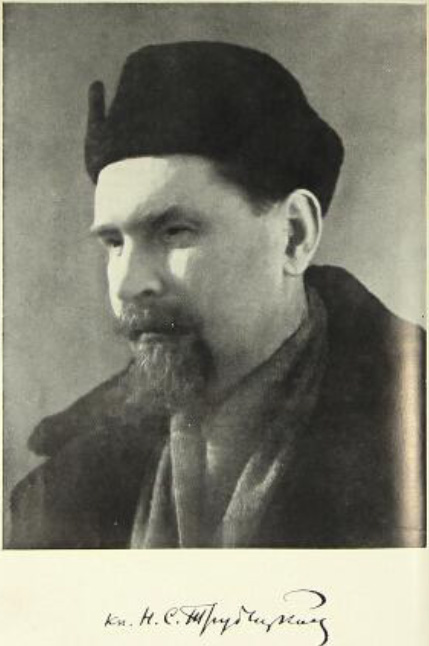
\includegraphics[width=.9\textwidth]{figures/Trubetzkoy_1939.jpg}
  \caption{Prince Nikolai Sergeievič Trubetzkoy}
  \label{fig:ch.prague_trubetzkoy_1939}
\end{wrapfigure}
In the \textsl{Grundzüge}, {\Trubetzkoy}'s discussion starts—with explicit
reference to the prior work of {\Saussure} and {\DeCourtenay}—from
the distinction between the \emph{Sprechakt}, or concrete act of
speaking, and the \emph{Sprachgebilde}. The latter is the system which
underlies, as a complex of socially determined values, actual concrete
acts of speaking: it is this system which enables these acts to
represent meanings for both the speaker and the hearer. Evidently, the
distinction between \emph{Sprechakt} and \emph{Sprachgebilde} is
largely the same in its essence as that between {\Saussure}'s
\emph{parole} and \emph{langue}.

On the basis of the fundamental difference between these two aspects
of the structure of a language (its material realization on the one
hand, and the system of distinctive values underlying this on the
other), {\Trubetzkoy} concludes that with respect to the study of sound
systems, two distinct disciplines must be kept separate. Phonetics, as
the science of sounds in their concrete physiological, acoustic, and
auditory aspects has quite a different object, and employs quite
distinct methods, from phonology or the science of the functional
distinguishing role of sounds within a \isi{linguistic system}. Of course,
these two disciplines are not totally separate, in that they refer to
one another's results. The phonetician pays more attention to the
material basis of those distinctions that have a linguistic function,
while the phonologist starts from the phonetic data showing that the
functional opposition between particular sounds is realized in such
and such a way. Aside from this sort of friendly `handshaking',
however, phonology as the science of the functional utilization of
sounds remains quite distinct in its goals and procedures from
phonetics.

The phonetician, in order to realize the ideal of this discipline,
must rigorously exclude from the investigation all reference to the
distinguishing, functional nature of speech sounds. Indeed, not even
the conventional \isi{segmentation} of speech is available to phonetics
\emph{a priori}, since it rests on the distinguishing function of
segments of sound; and this is of course notoriously difficult to
reconstruct \emph{a posteriori} on purely phonetic grounds. These
imperatives result in a necessarily atomistic study of particular
sound types, taken in isolation from one another except insofar as
they reveal similarities of formation or acoustic structure. The
phonologist, on the other hand, must make an equally rigorous effort
to limit attention to the strictly distinguishing properties of
opposed elements, observing the attendant nondistinctive properties
only long enough to reject their relevance as soon as they are shown
to have that character.

As a practical result of this separation, the systematic aspect of the
relations between the \isi{invariant} elements of the \isi{phonological system}
and the actual \isi{variation} found in phonetic form tends to fall between
two stools, and has no place in description. Phonology in these terms
only has room for a study of the \isi{invariant} \isi{representations}, and the
principles governing the systematic \isi{variation} in realization shown by
phonological elements have at best an uneasy place in the phonological
description (and none at all in phonetics). In consequence, the only
way to describe such systematic \isi{variation} is to incorporate it into
the definitions of elements of the phonological representation. We
will see this below in the notions of the \isi{archiphoneme} and of
\isi{neutralization}, and in the \isi{concept} of the morphophoneme.

In defining the basic elements of phonological structure, {\Trubetzkoy}
starts from the functional notion of opposition or \isi{contrast}. A
phonological opposition exists between two sound sequences when the
substitution of one for the other (perhaps within some large sequence)
results in a different \isi{meaning}. This may mean either a different word
or, to cover the case of accidental gaps, a sequence which represents
no word at all in the language under study. `Contrast' here clearly
means `\isi{contrast} on the surface': there is no provision for differences
between words other than those that are provided with a direct
phonetic implementation. In light of subsequent more abstract views of
phonology, we might be tempted to take this as a sort of empirical
claim about the range of differences that can possibly have linguistic
relevance, but to do so would be at the very least anachronistic. The
linguists of the Prague Circle and most of their contemporaries (with
a few isolated exceptions such as {\Sapir}, and despite the more
psychological orientation of {\DeCourtenay}) took it as
self-evident that if one wants to study the ways in which words are
differentiated from one another, the only conceivable starting point
is the overt phonetic manifestation of their differences.

Given two words that \isi{contrast}, we can presumably identify the phonetic
material in terms of which they differ. Such a stretch of sound is
called a `phonological unit'. For example, the \isi{contrast} between
\emph{phonological} and \emph{phrenological} allows us to isolate the
material represented by -\emph{o}- and -\emph{re}- in these words as
phonological units. When other pairs share subparts of these units,
this fact allows us to decompose them into smaller subunits. Thus, the
\isi{contrast} between \emph{Fred} and \emph{fraud} provides us with the
basis for decomposing -\emph{re}-into a sequence
-\emph{r}+\emph{e}-. When this analysis has been carried to the point
that the units arrived at cannot be further decomposed, the resulting
elements represent the phonemes of the language.

As we will discuss in chapter~\ref{ch.jakobson}, {\Jakobson} later argued
that a crucial misstep in this process is its limitation to the
decomposition of the sound material into a sequence of linearly
concatenated units. For him, the Saussurian conception of the sign as
essentially linear involves an erroneous limitation, and this must be
overcome by admitting also a decomposition of phonemes into their
simultaneously occurring components if the ultimate units of
phonological structure are to be uncovered. Such a further analysis is
not involved in {\Trubetzkoy}'s notion of the \isi{phoneme} though, and his
conception of the role played by the simultaneous distinctive
properties carried by this element is somewhat different from
{\Jakobson}'s.

{\Trubetzkoy} at first presents the process of analysis of sound material
into successively smaller constituents, based on functional contrasts,
as a definition of the \isi{concept} of `\isi{phoneme}'. It soon becomes clear,
however, that such an analysis serves a rather more limited role: it
merely reconstructs the phonetic \isi{segmentation} of the utterance (which
it will be recalled is not presumed by {\Trubetzkoy} to be available from
phonetic considerations alone), and still results in phonetically
`complete' elements, or `linguistic sounds'. These elements consist of
a vast range of properties, nondistinctive as well as distinctive, and
the phonological analysis must go further to separate the functional
wheat from the phonetic chaff if the ultimate contrastive units of
language are to be reached. What must be done, that is, is to identify
for each pair of `linguistic sounds' arrived at by \isi{segmentation}
whether or not they \isi{contrast} with one another, and, if they do, what
phonetic property provides the basis of this \isi{contrast}. The \isi{phoneme} can
then finally be defined as ``the sum of the phonologically relevant
particularities borne by a \isi{sound image}.''

It will be seen that the definitions thus given of the basic units of
phonological structure are couched in terms of analytic procedures
that could (in principle) be applied to objective phonetic data from a
given language in order to arrive at its inventory of phonemes—and not
in terms of some presumed antecedently given entity such as {\Baudouin}'s
``psychological equivalent of a \isi{speech sound},'' which must merely be
identified rather than reached as the end product of analysis. Partly
a product of the general climate of operationalism in science that
characterized the intellectual atmosphere of the 1930s when the
\textsl{Grundzüge} was written, this is also a consequence of the
{stress} put by {\Trubetzkoy} on the social rather than individual nature
of the \emph{Sprachgebilde}. If the \isi{linguistic system} is not a part of
any particular individual but, rather, exists as a set of social norms
or conventions among the members of a speech community (as {\Saussure}
had also argued), it follows that its essence cannot be either
physical phonetic or psychological.

In his earliest writings on phonological topics, {\Trubetzkoy} had in
fact made use of definitions of the \isi{phoneme} that rested on a
psychological foundation, partially under the influence of 
{\DeCourtenay}'s ideas on the subject. Indeed,
\citet{twaddell35:on.defining} lumps {\Trubetzkoy} together with other
proponents of the notion that the \isi{phoneme} is a ``mental or
psychological reality'' on the basis of the position taken in his early
important work on vowel systems \citep{trubetzkoy29:vowel.systems}. By
the time of the \textsl{Grundzüge}, however, he had come to reject
such a notion. This was partly because of his acceptance of a social
rather than an individual foundation for the \isi{linguistic system}, but
also in part (perhaps, indeed, primarily) because the psychological
definition appeared to give no basis for the analytic isolation of the
strictly distinctive properties of the \isi{sound image}.

As he notes, if we think of the `psychological image' of an intended
pronunciation, we have no reason to believe that this consists only of
its distinctive properties. Indeed, ``acoustic-motor \isi{representations}
correspond to each of the phonetic variants, to the extent that the
\isi{articulation} is controlled and regulated by the speaker. Neither is
there any reason to consider some of these \isi{representations} as
`conscious' and others as `unconscious'. The degree of consciousness
of the articulatory process depends only on practice. By special
training, one can become aware of the nonphonological properties of
sounds \ldots\ The \isi{phoneme} thus cannot be defined either as `phonic
representation' or as `conscious phonic representation' and thus be
opposed to the linguistic sound or the phonetic variant''
\citep[142]{trubetzkoy39:grundzuge}.

The operative term in this argument can be seen to be
`representation'. Evidently, so long as we confine our description of
the phonology of a language to the choice of a set of \isi{representations}
for utterances, the full set of acoustic-motor instructions apparently
entailed by the notion of a psychological image of intended
pronunciation will fail to distinguish distinctive from nondistinctive
properties. The anecdotal character of our actual awareness of
phonetic detail also contributes to make such consciousness far from
satisfactory. From this it appears to follow that an adequate
representation would have to be of a rather different nature, and that
the psychological conception of phonological structure must be
rejected. {\Trubetzkoy} relies here on the strongest form of the
proposition that a phonological theory is limited to being a theory of
\isi{representations}, and it is clear that his argument leads to a
conception of the \isi{phoneme} as a unit of such \isi{representations} consisting
of all \emph{and only} the distinctive properties of a given sound
segment.

In previous chapters, we have explored the possibility of attributing
significance within a phonological theory not only to the set of
\isi{representations} it provides for utterances, but also to a set of {rules}
that describe relations between them. On such a view, it would be
possible to maintain that the \isi{phonological representations} of
utterances include phonetic detail, either in the `fully specified
surface variant' form suggested in chapter~\ref{ch.saussure_sound} as
an interpretation of {\Saussure}'s position, or in the `specified basic
variant' form attributed in chapter~\ref{ch.kazan} to {\Baudouin} (and
even clearer for {\Sapir}; cf. chapter~\ref{ch.sapir} below). Within such
a theory, it would be possible to rehabilitate the psychological
conception of the \isi{phoneme}—at least as far as {\Trubetzkoy}'s argument is
concerned. Within the limitations implicitly placed by {\Trubetzkoy} on
the content of a phonological theory, however, his conclusion follows
that an adequate definition of the \isi{phoneme} must restrict the content
of these units to their phonologically distinctive properties.

While the \isi{phoneme} thus came to be identified with the sum of the
phonologically relevant properties of a sound, this does not at all
exhaust the content of the Praguian theory of phonological
structure. The most characteristic feature of this view, indeed, was
not the exclusion of nondistinctive properties (which the Prague
school linguists shared with most other positions at the time) but the
extent to which the \isi{phoneme} was regarded as embedded within a system
of structured \isi{oppositions}. The system of phonemes was not considered
as simply an inventory of building blocks of \isi{sound structure} from
which words could be constructed by concatenation, but rather as a
whole in which each element entertains specific and distinguishable
relations of fundamental importance with each of the other elements to
which it is opposed.

The study of such phonemic systems rests essentially on the
elucidation of the properties which underlie the \isi{oppositions} between
phonemes. For {\Trubetzkoy}, at least, these properties are phonetic
ones, and furthermore, by virtue of his rejection of a psychological
character for the system, they must also be properties which are
observably present in the speech signal. This position was rigorously
pursued to its conclusions: for instance, if the \isi{phoneme} is something
which is actually present in the speech signal, it must be the case
that a set of sounds can only be regarded as variants (or
realizations) of the same \isi{phoneme} if they share some unique subset of
phonetic properties which are not present together in any other sound
not belonging to that \isi{phoneme}. As something identifiable in principle
in the physical acoustic realizations of particular utterances, such
an externally construed, non-psychological \isi{phoneme} was directly in line
with the formal and socially based conception of language and
linguistics promoted by the Prague school.

It might well appear that if the \isi{phoneme} is something that can
actually be found by analysis in the speech signal, the substantive
side of such a phonological theory must reduce to an inventory of the
phonetic dimensions that are available to serve as the bases of
linguistic contrasts. Indeed, much of the \textsl{Grundzüge} is
devoted to a survey of such properties, giving examples of particular
languages in which they serve contrastively in order to demonstrate
their right to inclusion in a universal phonological theory. It is
important not to be misled by this, however, for an exhaustive
catalogue of potentially phonological parameters was pursued less as a
goal in itself than to make it possible to compare the systems of
different languages, to organize and classify the sets of \isi{oppositions}
obtaining within particular languages, and ultimately to state general
laws governing the structure of such systems and their role in
motivating and directing \isi{historical change}.

The ultimate goal of the Prague school theory of phonological
structure, then, was not simply descriptive in the sense of providing
an enumeration of all of the contrasts that could be observed
empirically in natural languages, though it included this project as a
subsidiary aim. Rather, it was explanatory, and intended to elucidate
general laws from which these empirical observations could be shown to
follow. For example, by relating both \isi{oppositions} of \isi{pitch} (\isi{tone}) and
those between palatalized and non-palatalized \isi{consonants} to a single
dimension of `tonality', {\Jakobson} and {\Trubetzkoy}
(cf. \citealt{jakobson29:remarks}\footnote{{English} transation with
  extensive annotations by \name{Ronald}{Feldstein},
  \protect\citealt{jakobson18:remarks}.}) came to the conclusion that
no language could display these two contrasts simultaneously and
independently. When this observation is raised to the status of a
`law' governing phonological systems, we predict, for example, that
when a language develops the opposition of \isi{palatalization}, it must
subsequently lose any independent tonal (\isi{pitch}) contrasts---a claim
that \citet{jakobson29:remarks} saw as borne out in the history of
Slavic. The particular claim here is not actually valid, since there
exist languages such as the \ili{Szechuan Chinese} dialect studied by
\citet{scott56:szechuanese} in which \isi{palatalization} and tonal
contrasts are independent; but this does not alter its value as
illustrative of the aims (if not necessarily the accomplishments) of
Praguian phonology in the domain of phonological \isi{explanation}.

\section{The structure of phonological systems}
\label{sec:structure-of-systems}

While phonemic systems are founded in {\Trubetzkoy}'s view on physical
properties of the sounds that realize their elements, the analysis of
a particular system does not reduce to a simple task of phonetic
description. In general, it is not possible to tell from the phonetic
properties of a segment in isolation (even given a universal inventory
of potentially distinctive parameters such as that proposed in the
\textsl{Grundzüge}) just how it should be characterized phonemically. This is
because it is not merely its phonetic identity that matters
phonologically but, more importantly, what other segments it is
opposed to in the language in question. 

In \ili{English}, for example, we find \isi{stops} at labial, dental, and velar
positions that are quite parallel phonetically. Nonetheless, their
phonemic content is not similarly parallel. If we consider /t/, for
example, we can see that this segment is phonologically
\emph{voiceless} (because it is opposed to /d/), \emph{non-nasal}
(because opposed to /n/), \emph{dental} (because opposed to /p/ and
/k/), and a \emph{stop} (because opposed to /s/ and to /ɵ/). In
\isi{contrast}, /k/ is \emph{voiceless} (because opposed to /g/),
\emph{non-nasal} (because opposed to /ŋ/), and \emph{velar} (because
opposed to /p/ and to /t/); but given the absence of a velar
continuant /x/ in \ili{English}, /k/ is not \emph{phonologically} a stop. Of
course it is not a fricative either: it is simply not specified in any
way for this property (though the phonetically similar /p/ and /t/ are
both specified as \isi{stops}).

Indeed, even knowing the range of segments to which a given \isi{phoneme} is
opposed does not make its phonological analysis self-evident. This is
because any given opposition may provide a number of potential
dimensions simultaneously, along any one of which the \isi{contrast} might
be established. The requirement that all non-distinctive properties
must be eliminated, however, means that not all of these features can
be simultaneously present in a given \isi{phoneme} (assuming they
co-vary). For example, in considering vowel systems, we often find
(among the non-low vowels of a language) a \isi{contrast} between /u/ and /o/
on the one hand, and/i/ and /e/ on the other. These differ in terms
both of rounding and of backness, and we must establish in each
particular case which of these properties is the phonologically
relevant one.

The answers to such questions are found in the interaction of
language-parti\-cu\-lar factors with general laws governing the
structure of phonological systems. In \ili{Russian}, for example, when we
consider the \isi{phoneme} /i/, we find that it may be phonetically either
front {[i]} or mid-back {[ɨ]}, depending on its consonantal
environment. Similarly, /u/ is phonetically less back after certain
\isi{consonants} than after others. Since frontness is not invariably
present in the realizations of /i/ and absent in realizations of /u/,
it follows that the two must be opposed to each other in rounding
instead.

{\Trubetzkoy} contrasts this state of affairs with that obtaining in
\ili{Japanese}, a language which also has the vowels /i, /e/, /u/, /o/ and
/a/. In \ili{Japanese} there is a \isi{contrast} between palatalized and
nonpalatalized (dental) \isi{consonants} which appears before the vowels
/a/, /o/ and /u/; before /i/ and /e/, however, only the palatalized
segments appear. On the basis of this regularity, {\Trubetzkoy} argues
that /i/ and /e/ must be opposed to /u/ and /o/ in terms of backness
rather than rounding. This follows from the further fact that /a/
(which patterns like /u/ and /o/ in this respect) is back, but not
round.

A parallel argument bearing in the opposite direction is based on the
facts of \ili{Northern Ostyak}: in this language, the vowels /u/, /o/, /ɔ/
only occur in initial syllables, while the vowels /a/, /ɛ/, /e/ and /i/
appear in non-initial syllables as well. Since /a/ (which is
phonetically back as well as unround) patterns like the other
non-round vowels rather than like the other back vowels, {\Trubetzkoy}
concludes that the /i/-/u/ opposition in this language is based on
rounding rather than on backness.

In other languages, other facts resolve similar questions. In many
languages with /i/, /e/ and /u/, /o/, for example, we find more than
one low vowel. When we find a back unrounded /ɑ/ and a front unrounded
/æ/, as in certain Montenegrin dialects of \ili{Serbo-Croatian}, we can
identify the \isi{contrast} as one of backness (in the non-low as in the low
vowels). On the other hand, when we find a back unrounded /ɑ/ and a
back rounded /ɔ/, we must treat the \isi{contrast} of /i/ vs. /u/ as one of
rounding on the \isi{analogy} of the only possible account of the \isi{contrast}
in the low vowels.

Such arguments make an implicit appeal to a principle which has since
been taken as absolutely fundamental to the choice of a set of
phonological dimensions in a universal theory: the notion that the
features defined by such a set ought to facilitate the definition of
`natural classes' whose relevance is displayed by some common behavior
shown by their members as opposed to nonmembers of the class in
question. {\Trubetzkoy} never articulates this principle as an explicit
basis for the choice of one possible proposed feature over another in
analyses, but he makes constant implicit appeal to it in the decisions
he makes and in the way he uses particular examples to support his
choices such as those just reviewed.

We have noted that much of the \textsl{Grundzüge} is devoted to a
presentation of a putatively exhaustive set of phonetic dimensions
along which phonological contrasts can be established in any natural
language. This presentation is intended to serve as a descriptive
framework for the higher purpose of developing a substantive
phonological theory: in particular, the development of universally
valid laws governing the structure of phonemic systems.

The first step in describing such systems is to establish the set of
phonemes which \isi{contrast} in the language, and {\Trubetzkoy} presents a set
of explicit procedures for accomplishing this. Some of these
procedures, such as the tests for whether a given stretch of phonetic
material should count as a unitary \isi{phoneme} or as a sequence of two—for
example, the choice between \isi{affricates} and sequences of \isi{stops} plus
\isi{fricatives}—are somewhat \emph{ad hoc} and ultimately unsatisfactory,
as has been argued in the subsequent literature; but it must be
admitted that the problems they address are among the classic
chestnuts of the field, and that subsequent work cannot be said to
have solved them to general satisfaction.

In any event, there is a difficulty of principle here. In {\Trubetzkoy}'s
account of phonological structure, this is strictly an external
construct, based on a social reality and arrived at by a set of fixed
procedures. There is in fact no sort of `external' evidence which
could count as confirming or disconfirming particular analyses, and it
is difficult to argue convincingly that a given procedure or use of
language-internal evidence, as in the establishment of \isi{oppositions} in
the fashion described in the preceding paragraphs, yields incorrect
results—except on the basis of æsthetics or a sort of presystematic
intuition of what the solution `must be'. The extent to which any
external evidence exists to confirm a given solution is another of the
standard problems of phonology, and of course it is by no means
uniquely a problem for {\Trubetzkoy}'s views. It exists there
nonetheless, and perhaps in an exacerbated form as a result of the
extent to which he separates the \isi{phonological system} from any other,
independently verifiable, aspect of language.

Having established the set of contrasting phonemes, the analyst next
asks about the nature of the \isi{oppositions} among them. It is the
totality of these \isi{oppositions} that yields the \isi{phonological system} of
the language. Since any two phonemes (and not simply those that differ
in only one or two properties) must be regarded as opposed to each
other, many of these \isi{oppositions} are based on quite a few
phonologically relevant properties at once.

Of course, if all pairs of phonemes differed in an essentially global
way, the resulting system would be no different in substance from a
simple inventory. Interestingly, however, some \isi{oppositions} are based
on only one property or some small number of related properties, and
sometimes some one property serves as the (only) distinction within
more than one pair of opposed phonemes. It is this kind of opposition
that gives phonological systems an interesting internal structure, and
it is the analysis of this kind of structure that led
\citet{jakobson28:first.icl} to emphasize in his propositions for the
First International Congress the search for `\isi{correlations}' or
recurrent \isi{oppositions} that allow the decomposition of other
alternations into component parts.

For the interpretation of such structure, {\Trubetzkoy} proposes that
\isi{oppositions} can be classified along several simultaneous
dimensions. For instance, \isi{oppositions} can be distinguished between
those that are \emph{isolated} in that exactly the same combination of
features does not serve to distinguish any other pair of phonemes in
the language and those that are \emph{proportional} (or
recurrent). Most phonemes in a given language, taken pairwise, will as
already remarked form isolated \isi{oppositions}. In \ili{English}, for example,
the opposition between /m/ and /d/ is isolated, since the combination
of features in which they differ (a labial nasal vs. a voiced dental
stop) does not recur as the basis of any other opposition in the
language. It is the proportional \isi{oppositions} that are of special
interest, such as that between \ili{English} /p/ and /b/ (whose difference,
\isi{voicing}, reappears as the minimal difference between /t/ and /d/, /s/
and /z/, etc.).

We can also distinguish between \emph{bilateral} and
\emph{multilateral} \isi{oppositions}. When the same phonetic property
distinguishes more than two phonemes along the same dimension, the
resulting opposition is a multilateral one. {\Trubetzkoy} treats place of
\isi{articulation} as a single dimension, and thus /p/ vs. /t/ vs. /k/
constitutes a multilateral opposition if we assume these phonemes do
not differ in any other feature. When exactly two phonemes are
distinguished minimally on a given dimension, though, we have a
bilateral opposition such as \isi{voicing} in \ili{English} (since there is no
third value other than `voiced' and `unvoiced' , holding other
properties constant). As we will see in chapter~\ref{ch.jakobson},
{\Jakobson} differed from {\Trubetzkoy} on the question of whether any
\isi{oppositions} are in fact multilateral, but {\Trubetzkoy}'s framework
includes at least some properties that could serve as the basis of
multilateral \isi{oppositions}.

Additionally, it is possible to distinguish \isi{oppositions} in terms of
their `logical' character. When two phonemes differ in that one
contains a particular property which is lacking in the other,
{\Trubetzkoy} calls such an opposition a \emph{privative} one. The
opposition between phonemes with and without an added nasal resonance,
for example, is privative. In \isi{contrast}, when two phonemes differ in
that they contain different properties (rather than one simply having
a property that the other lacks), the opposition is \emph{equipollent}. The
difference between vowels with and without rounding, for example, is
generally to be regarded as privative, while that between front and
back vowels is equipollent. A final possibility of this sort is a
\emph{gradual} opposition, in which both phonemes possess a given property
but to varying degrees. The opposition between mid and high vowels for
instance is generally a gradual one based on their relative degree of
openness.

There is further subdivision of the types of opposition in the
\textsl{Grundzüge} and other work of {\Trubetzkoy} and the Prague school,
but the basic categories above should give the flavor of the types of
classification proposed. It is interesting to note that despite the
amount of effort expended on such definitions and distinctions among
types of opposition, the resulting \isi{typology} plays hardly any role in
the theory. The proposed laws of phonological structure generally make
no reference to \isi{oppositions} by type but are, rather, based on the
specific substantive content of particular \isi{oppositions}.

Among these laws, for example, is the proposal that if a language
distinguishes between a set of `bright' (front and/or unrounded)
vowels and a set of `dark' (back and/or rounded) vowels, either the
two sets have the same number of elements, or there is exactly one
vowel which is neutral between them, and this is the most open vowel
in the system. If the language further distinguishes a third class
intermediate between the `bright' and the `dark' vowels (e.g. a set of
central unrounded or front rounded vowels), there cannot be more
members in this set than in the set of `bright' vowels. Such
principles make no essential use of the logical classification of
\isi{oppositions}, but only of their substantive content.

There is one partial exception to this: a class of \emph{correlations}
is defined from the earliest writings of the Prague phonologists,
which in {\Trubetzkoy}'s work is characterized as the set of
proportional, bilateral, privative \isi{oppositions}. The \isi{correlations} have
a unique role to play in the description of what we would now
interpret as morphophonemic phenomena, especially those connected with
the notion of \isi{neutralization}. We will return to these questions in
section~\ref{sec:neutralization}.

\section{Suprasegmental properties}

{\Trubetzkoy}'s survey of phonological contrasts in natural languages and
his proposed set of parameters for a general theory constitute the
foundation of subsequent efforts to delimit such a universal set of
features. For the most part, the actual dimensions he discusses are
rather traditional ones, though the addition of acoustic terminology
in some definitions had consequences that were unfamiliar at the
time. It would take us too far afield to discuss his proposals in
detail here, but in one respect we must at least sketch his views,
since they constituted innovations in an area which was only somewhat
later rediscovered within generative phonology.

The bulk of the proposed phonological features in the
\textsl{Grundzüge} relate to properties of the traditional phonetic
segment, and the fundamental status of this unit in {\Trubetzkoy}'s view
of phonological structure is beyond question. Nonetheless, he also
devotes considerable attention to properties whose association with
segmental structure is at best loose. This is a real departure in
Prague school theory from previous accounts of phonology, and these
were the first linguists in a modern sense to devote really serious
attention to the domain of `prosodic' features. This was actually a
rather natural outgrowth of the attention paid by the originators of
Praguian theory (especially {\Jakobson}) to problems of poetic structure
as the original inspiration for their interest in language.

{\Trubetzkoy}'s theory of prosodic features is based on the insight that
some properties naturally appertain not to particular segments but to
entire syllables. He sketches a view of the structure of syllables,
which are constructed around an obligatory \isi{nucleus} made up typically
of a vowel or vowels (but in some languages also including certain
consonantal elements). He then argues that while properties such as
distinctive \isi{tone} are typically realized as part of the \isi{articulation} of
the segment(s) making up the \isi{nucleus}, it is an error to treat them as
properties of these segments themselves. Rather, he says, they are
properties of the \isi{syllable}, with the peculiarity that they are
realized in a particular portion of the \isi{syllable}'s structure.

Beyond recognizing the \isi{syllable} as the locus of assignment of \isi{tone} and
accentual properties, {\Trubetzkoy} also recognizes that the role played
by a segment within a \isi{syllable} may itself constitute a distinctive
phonological dimension. Here what is in question is the difference
between `syllabic' and `non-syllabic' forms of what is otherwise the
same segment type. The former make up part of the \isi{nucleus} while the
latter do not, but there may be no other independent property
distinguishing them beyond that of their integration into syllabic
structure (a point that had been made before by others, including
{\Saussure}; cf. chapter~\ref{ch.saussure_sound}). This is the case, for
example, with the difference between high vowels such as /i/ and /u/
and the corresponding semivowels /j/ and /w/, and also with the
syllabic (vs. nonsyllabic) resonants like /r̩/ and /l̩/ that are found
in some languages (\ili{Czech} and \ili{Serbo-Croatian}, for example). Sometimes
even obstruents may be syllabic, as {\Trubetzkoy} argues for \ili{Mandarin
Chinese}.

In many cases the difference between syllabic and non-syllabic forms of
a segment may be completely predictable and thus non-phonological,
when it is entirely determined by the consonantal environment for
example, but in other languages the same phonetic difference may be
independently contrastive. As with the earlier discussion of the
identification of phonemic contrasts, he gives a number of procedural
principles for deciding when apparently syllabic \isi{consonants} should be
analyzed as displaying the `correlation of syllabicity' and when they
should be treated as sequences of a reduced vowel and a non-syllabic
consonant. The exact content of these {rules} is not particularly
interesting in itself; they are not free of the \emph{ad hoc} nature of other
such procedurally oriented definitions, and probably raise as many
problems as they answer. What is significant is the recognition that
among the properties that may have phonological relevance are some
that cannot be assigned to the segment itself in any natural way, but
rather reflect the distinct ways in which one and the same segmental
content may be integrated into a larger structure (the \isi{syllable}).

This notion plays a particularly important role in {\Trubetzkoy}'s
account of the nature of linguistic quantity, to which he devotes a
good deal of attention. He notes first of all that while many
languages have a \isi{contrast} among long and short vowels, this \isi{contrast}
may have very different status in different systems. He then argues
that while such length is often to be treated as a (segmental)
feature, there are also cases in which a long vowel ought rather to be
regarded as composed of two (or, at least theoretically, even more)
sub-units called moras.

A number of circumstances are cited in which such decomposition of
long vowels is warranted. Most obviously, this may be the case when
(at least some of) the long vowels in a language arise from the
juxtaposition of two morphological elements, the first of which ends
in a vowel and the second of which begins with one; or from the loss
of intervocalic \isi{consonants}, leading to sequences of identical vowels,
etc. Besides such cases, where the compound nature of the resulting
long vowel is patent, however, it is also possible to argue for a
similar decomposition on other grounds. For instance, if a language
contains some diphthongs which are analyzed as vowel sequences, and
the long vowels of the language display some important similarity of
behavior with these diphthongs such as attracting the \isi{stress}, then it
is justifiable to treat them as `diphthongs' made up of two identical
elements.

Again, it may be the case that certain prosodic \isi{oppositions} are
limited to syllables containing long vowels or diphthongs, in which
case the treatment of long vowels as made up of two (or more) moras is
also indicated. In \ili{Lithuanian}, for example, long syllables can bear
either falling or rising \isi{accent} (or be unaccented), while short
syllables only \isi{contrast} as accented vs. unaccented. Treating the
difference between rising and falling \isi{accent} as a matter of which mora
in a long \isi{syllable} bears the \isi{accent} allows a simple and natural
account of this complex accentual system, justifying the decomposition
of the long vowels.

Not all languages in which long and short vowels \isi{contrast} provide
evidence of the sort {\Trubetzkoy} regards as warranting the analysis of
the long vowels into moras, however, and in other cases we must regard
such a \isi{contrast} as a simple one of `intensity' applying to a single
segment. The same phonetic material (a long vowel) may thus be
analyzed differently in different languages, depending on whether it
represents simply a segment with a particular property (increased
intensity) or the integration into a single syllabic \isi{nucleus} of two
distinct but segmentally identical moras.

A third phonological interpretation of phonetic quantity distinctions
is also proposed, which is even more interesting from the point of
view of \isi{syllable} structure. In some languages, he suggests, the
difference between long and short vowels depends not on a property of
the vowels themselves but on whether the vowel is `free' in its
\isi{syllable} or `checked' by a following consonant. It might appear that
what is involved in the `correlation of close contact' (or
\emph{Silbenschnittkorrelation}) is simply a matter of the difference
between vowels in open and in closed syllables, but it is evident from
the examples he gives that this is not what {\Trubetzkoy} has in mind.

Central among these is the case of \ili{Hopi}, which appears (on the basis
of observations by {\Whorf}) to show not two but three degrees of vowel
length. A minimal set of three forms displays this \isi{contrast}: [păs]
`very' with extrashort vowel; [pas] `field' with middle quantity; and
[pās] `calm' with a fully long vowel. From the fact that all three of
these forms are monosyllables ending in a consonant, and thus closed
syllables by any natural criterion, it is clear that a simple
difference between open and closed syllables is not what is at issue
here.

\begin{figure}[ht]
  \begin{centering}
    \begin{forest}
      [σ [onset[p]] [\isi{nucleus} [a][s]]]
    \end{forest}
    \begin{forest}
      [σ [onset[p]] [\isi{nucleus} [a]] [coda[s]]]
    \end{forest}
    \begin{forest}
      [σ [onset[p]] [\isi{nucleus} [a][a]] [coda[s]]]
    \end{forest}
  \end{centering}
  \caption{păs `very' \emph{vs.} pas `field' \emph{vs.} pās `calm' in Hopi}
  \label{fig:ch.prague_silbenschnitt}
\end{figure}

{\Trubetzkoy} argues that two separate \isi{oppositions} are at work in
\ili{Hopi}. One of these is a \isi{contrast} between long and short vowels on the
basis of the difference between two moras and one: the longest vowel
quantity (that of [pās] `calm') differs from the other two in that it
involves a bimoric long vowel while the others contain only a single
mora. But in that case, how are we to distinguish [păs] `very' from
[pas] `field'? This, he claims, is based on whether the following
consonant interrupts (checks) the \isi{articulation} of the vowel or not—a
matter of whether the consonant itself is incorporated into the
\isi{nucleus}. We could represent the difference structurally as in
figure~\ref{fig:ch.prague_silbenschnitt}, employing the notation used
in the generative literature for describing the internal constituency
of syllables (though {\Trubetzkoy} himself does not propose a graphic
representation of the \isi{contrast}):

Other \isi{representations} of this analysis could be imagined (see
\citealt{sra84:halle-fest-II} for further discussion of this and other
claims of {\Trubetzkoy} and {\Jakobson} about the treatment of quantity as
they might be interpreted in the framework of Metrical Phonology), but
the essential aspect is the treatment of a postvocalic consonant as
distinctively falling either within or outside the \isi{nucleus} of its
\isi{syllable}. In \ili{Hopi}, this is argued to provide an immediate account of
the absence of the extrashort quantity in open syllables, where there
is no consonant available to check the vowel. The absence of a free
vs. checked \isi{contrast} in the genuine (bimoric) long vowels suggests the
rather natural constraint that no more than two units can appear in a
single \isi{nucleus}: either two vowel moras (yielding the greatest length)
or one vowel and one consonant (yielding the shortest).

{\Trubetzkoy} argues that the \emph{Silbenschnittkorrelation} is the
basis of length contrasts in a number of languages, including \ili{English}
and \ili{German}. For our purposes, the greatest interest of this proposal
lies not in the analysis of individual languages, however, but in the
theoretical innovation it involves. One and the same sequence of
phonemic units is here allowed to compose both members of a pair of
contrasting forms which differ exclusively in the way in which this
material is organized into higher-level units.

Had subsequent research pursued the substantially enriched conception
of phonological structure on which this proposal is based, there might
have been important consequences. In general, though, phonologists
maintained until late in the century a notion of \isi{representations} as
composed simply of a linear sequence of discrete, homogeneous
segments. Discussion of the \isi{syllable} was not of course completely
lacking, and the British school of \isi{prosodic analysis} in particular
discussed the notion of phonological properties that inhere in the
\isi{syllable} and its internal organization (see
chapter~\ref{ch.firth}). It does not seem unfair to say, however, that
no thoroughgoing integration of segmental and syllabic structure was
developed as the basis of a theory of phonological structure until the
advent of \isi{metrical phonology} in the 1970s (see
chapter~\ref{ch.otlabphon} below).

Within the scope of more orthodox prosodic features, {\Trubetzkoy}
presents a rather restrictive theory of tonal distinctions. He first
makes it clear that the phonological significance of the \isi{pitch} of a
given segment lies in its relative and not its absolute value. This
point, by now so familiar to phonologists as to seem self-evident, has
significant consequences for an understanding of the nature of
phonological distinctions in general, and it provided an eloquent
demonstration of the superiority of the phonological perspective over
the purely phonetic in analyzing particular languages.

At the time {\Trubetzkoy} wrote, even rather sophisticated observers of
tonal phenomena such as \citet{doke26:zulu} in his work on Zulu
tended to get mired in largely irrelevant detail, since they
concentrated on the measurable phonetic facts of \isi{pitch} rather than on
the phonologically more significant question of what tonal
possibilities existed contrastively in a given environment. By
concentrating his attention on the relative \isi{pitch} distinctions that
operate in particular positions, {\Trubetzkoy} brought much more clarity
to the analysis of \isi{tone}. In the process, he demonstrated the
fundamental difference between a phonological property (e.g., `high
\isi{tone}') and its phonetic realization (which might be anywhere within a
very wide range of actual \isi{pitch} values).

{\Trubetzkoy} distinguishes in his account between `\isi{tone} register'
contrasts (differences in simple relative \isi{pitch}) and `\isi{tone} movement'
contrasts (such as that between a rising and a falling \isi{tone}). The
latter are recognized only for languages in which long vowels exist,
and are analyzed into sequences of moras. In this way he ultimately
reduces the inventory of available \isi{tone} features to a set of relative
\isi{levels}, since he can then analyze a falling \isi{tone} as a sequence of a
relatively high \isi{tone} on the first mora of a long vowel followed by a
relatively lower \isi{tone} on the second mora, with a rising \isi{tone} being
represented as the reverse sequence. By admitting only (logically)
level \isi{tone}s, he succeeds in tremendously simplifying the range of
possible \isi{tone} systems.

Further simplification results from his claim that only three tonal
registers need be recognized phonologically in any given language: a
`normal' register, and \isi{tone}s either above this or below it in relative
value. Where more \isi{tone} registers appear to exist, he argues that they
are illusory. The additional values are either the result of
non-distinctive phonetic modification, as when a low \isi{tone} on a final
\isi{syllable} is lower than low \isi{tone}s elsewhere, or else some additional
distinction such as a difference in voice quality is
operative. Similarly, some apparently non-stationary \isi{tone}s are argued
to be either non-distinctive variants of basically level \isi{tone}s, or the
consequence of some other dimension interacting with voice \isi{pitch}.

Both of these major factual claims of his system, that phonologically
non-level \isi{tone}s can only occur on bi-moraic vowels and that three tone
\isi{levels} are sufficient to describe all languages, can be shown to be
false (see \citealt{sra78:tone_features} for a summary and
references). It has been demonstrated, in particular, that contrastive
\isi{tone} contours in some languages can occur on phonologically short
vowels. Nonetheless, the development of a notion of tonal
representation as `autosegmental'—i.e., as partially independent of
segmental structure—would allow us to maintain the essence of
{\Trubetzkoy}'s claim, which is the proposal that contour \isi{tone}s can
always be decomposed into sequences of \isi{levels} and need never be
recognized as primitives of a tonal feature system.

{\Trubetzkoy}'s system for the description of \isi{tone}s is quite close in
spirit to ones accepted today. This is especially true if one takes
literally the claim at the beginning of his discussion of prosodic
properties that features like \isi{tone} are associated not with segments on
a one-to-one basis but, rather, with larger units such as the
\isi{syllable}. If this view is consistently worked out, the supposed
dependence of \isi{tone} contours on the complexity of the \isi{syllable} \isi{nucleus}
is seen not to be a necessary consequence of other aspects of
structure (though it would of course be interesting if it were true)
but rather an empirical claim which turns out to be false.

In a number of regards, {\Trubetzkoy}'s position can be clearly
distinguished from that of other early phonological accounts of \isi{tone}
in the United States in the 1940s and 1950s, such as {\Sapir}'s work and
especially that of \citet{pike:tone_lgs}. These analysts differ from
{\Trubetzkoy} in recognizing both contrastive tonal contours (distinct
from sequences of \isi{levels}) in some languages, and a larger number of
\isi{levels}. In the latter claim they appear to be validated by the
existence, of languages in which at least four, and possibly five,
tonal \isi{levels} cannot be further reduced (see
\citealt{sra78:tone_features} for references); but with reference to the
structurally more interesting claims concerning contour \isi{tone}s,
{\Trubetzkoy}'s position seems at minimum to be a defensible one.

Within his study of prosodic properties, {\Trubetzkoy} proposes a number
of potentially general laws governing the structure of phonological
systems, in line with the Prague school program of formulating such
principles as the ultimate aim of a phonological theory. Some of these
can be seen to be logical consequences of the framework in which they
are formulated: for example, the claim that \isi{tone}-movement contrasts
only occur in languages in which the long vowels are analyzed into
moras follows largely from the fact that the very existence of such
contrasts provides sufficient evidence to require the decomposition of
long vowels into moras. Others, however, such as the proposal that
languages cannot display simultaneously a \isi{contrast} of freely
distributed (\isi{stress}) \isi{accent} and freely distributed quantity (aside
from the \isi{contrast} between `free' and `checked' vowels, which does not
count as `quantity' in the relevant sense), seem to be genuine
empirical propositions.

This proposed incompatibility of free \isi{stress} and free quantity (which
dates back to \posscitet{jakobson28:first.icl} proposals at the first
{International Congress of Linguists}) elicited a considerable amount of
discussion devoted to either disproving it or showing that it followed
from other principles. It is possible to argue that when the notions
of `free \isi{stress}' and `free quantity' are properly formulated within
the framework of \isi{metrical phonology}, the generalization proposed by
{\Jakobson} and {\Trubetzkoy} follows as a theorem from independent
properties of the two \citep{sra84:halle-fest-II}. At minimum, we must
regard this generalization as a fruitful hypothesis.

\section{Neutralization, archiphonemes, and markedness}
\label{sec:neutralization}

We return now to the formal (rather than substantive) nature of the
phonological theory presented in the \textsl{Grundzüge}, and in
particular to the dimensions along which this theory classifies
phonemic \isi{oppositions}. In addition to the parameters of this sort which
we discussed above, there is one more which is of fundamental
importance for {\Trubetzkoy}'s views: the difference between \isi{oppositions}
that are \emph{constant} and those that are \emph{suspensible}. If the
opposition between the members of a particular pair of phonemes is
constant, this means that either one can appear (in \isi{contrast} with the
other) in any environment. Suspensible \isi{oppositions}, on the other hand,
are those for which there is at least some environment in which the
two phonemes involved cannot \isi{contrast} with each other. In such a
position, the opposition between the two is said to be
neutralized. For example, in \ili{Russian} or \ili{German}, only the voiceless
members of voiced/voiceless pairs appear in final position, where they
thus do not \isi{contrast} with the corresponding voiced segments. We say,
then, that the opposition of \isi{voicing} (a correlation, in terms of the
classification discussed above) is neutralized in this position in
these languages.

Where an opposition is neutralized, we can then ask what the phonemic
entity is that appears in the position of \isi{neutralization}. Taking the
case of \ili{Russian} or \ili{German} final voiceless obstruents as a concrete
instance, we can note that in both languages, phonemes such as /p/
vs. /b/, /t/ vs. /d/, etc., can be identified in positions where
\isi{voicing} is not neutralized, but what of the phonetic [p], [t], etc.,
that occur finally? If we assume that no other neutralizations are
involved, these apparently have all of the phonological properties of
other instances of /p/, /t/, etc—except that, since they are not
opposed to voiced segments, they cannot contain any value for the
property of \isi{voicing} (by the definition of the \isi{phoneme}, since no such
value would be distinctive in this position). As a result, such an
element must consist of exactly the features common to /p/ and /b/,
/t/ and /d/, etc., but lacking the feature which elsewhere separates
the members of these pairs.

Such an element, identical with the subset of features common to a
pair of phonemes whose opposition is neutralized in some position, is
called by {\Trubetzkoy} an \emph{archiphoneme}. The existence of
archiphonemes is an immediate consequence of the possibility that
\isi{oppositions} may be suspended in certain positions, together with the
definition of the \isi{phoneme} as consisting of all and only the properties
that distinguish it from other elements of the system. For {\Trubetzkoy},
the archiphonemes in a system constitute additional elements of the
system beyond the inventory of phonemes: thus, the system of \ili{German} or
\ili{Russian} contains the \isi{archiphoneme} /P/ (representing the features
common to /p/ and to /b/) as well as the individual phonemes /p/ and
/b/. Since archiphonemes are essentially related to (and indeed
implied by) independently established \isi{oppositions}, however, they are
not generally presented as distinct units in phonological systems.

Since archiphonemes are implied by the \isi{neutralization} of particular
\isi{oppositions} between segments which are non-distinct along all other
dimensions, and since they are themselves phonemic entities, it
follows that only certain pairs of phonemes can have a corresponding
\isi{archiphoneme}. In particular, the segments involved must share some set
of common properties which distinguish them from all other elements of
the system. Thus, for example, an \isi{archiphoneme} /P/ representing the
\isi{neutralization} of /p/ and /b/ in final position in \ili{German} is possible,
since its content (the features common to /p/ and to /b/) is that of
an `oral labial stop', properties which set it apart from any other
\isi{phoneme} in the language. Even though /h/ and the velar nasal /ŋ/ do
not \isi{contrast} anywhere in \ili{English}, however, an \isi{archiphoneme}
representing the two is impossible since the only feature they have in
common is that of `consonant', and there are of course many other
\isi{consonants} from which this element would not be distinct.

In his definition, {\Trubetzkoy} argues that only bilateral \isi{oppositions}
can be neutralized and thus represented by an \isi{archiphoneme}. His claim
here is based on a logically incorrect argument, however. He reasons
that if, in \ili{German}, only /b/ and not /d/ appears before /l/, it is
still not possible to say that the opposition between /b/ and /d/ is
neutralized and represented by an \isi{archiphoneme} in this position, since
such an \isi{archiphoneme} could only be identified as `voiced oral stop',
and there is another voiced oral stop in the system (/g/) from which
it would thus not be distinct. From this it can be seen that a proper
subset of the segments involved in a multilateral opposition cannot be
represented by an \isi{archiphoneme} without destroying the distinctness of
this unit from the other elements of the same opposition.

While this argument does indeed show that not all instances of the
apparent suspension of a multilateral opposition can be coherently
represented by an \isi{archiphoneme}, it certainly does not suffice to show
that no multilateral \isi{oppositions} are so neutralized: it is simply
necessary to be sure that the entire opposition is effectively
neutralized in a given case, and not just a proper sub-part of
it. Consider the common case of a language which, in pre-vocalic
position, contrasts several \isi{nasal consonants} (along the multilateral
dimension of \isi{place of articulation}), but in which pre-obstruent nasals
must always be homorganic with the following consonant. Surely in such
a language we would want to say that an \isi{archiphoneme} /N/ (defined
simply as `\isi{nasal consonant}') represents the multilateral opposition in
the position of \isi{neutralization}. Such an element is completely well
formed by all of the other defining criteria for archiphonemes.

Assuming that any phonological opposition can be neutralized and
repre\-sented by an \isi{archiphoneme} in particular environments, then, so
long as the resulting \isi{archiphoneme} remains distinct from all other
contrastive phonemic elements occurring in the given position, the
next question is that of the phonetic realization of such
elements. {\Trubetzkoy} notes that an \isi{archiphoneme} may be represented by
a segment identical with other realizations of one or the other of the
phonemes involved (as with the case of the final voiceless \isi{stops} which
represent \ili{German} or \ili{Russian} obstruent archiphonemes), or its phonetic
realization may be different from any segment that occurs in other
positions. This is the case, for example, with the voiceless
unaspirated \isi{stops} which appear in \ili{English} as the realization of
neutralized obstruents /P/, /T/, and /K/ after /s/. The one thing
which is determinate, of course, is that the realization of the
\isi{archiphoneme} must contain the properties which define it; that is,
which are common to the neutralized phonemes it represents.

This notion that the \isi{phonological identity} of a segment may be
determined only relative to a particular environment is one which is
not unique to Prague school phonology. As we will see in
chapter~\ref{ch.firth} below, it constitutes the central tenet of
Firthian `polysystemic' analysis, and a central reason behind the
rejection of phonemic analysis altogether by his school. In the
context of American \isi{phonemic theory} (which we will discuss in
chapter~\ref{ch.structuralists}), \citet{twaddell35:on.defining} had
arrived at rather similar notions by a completely different route, as
{\Trubetzkoy} recognizes in a passage of the \emph{Grundzüge}. Taking
into account simply the distribution of individual phonetic segments,
{\Twaddell} had observed that the range of distinctions present in some
positions is quite different from that in other positions, and thus
that the distinctive value of the same segment under different
environmental conditions may be quite different. {\Twaddell}'s
terminology is quite different from {\Trubetzkoy}'s (or {\Firth}'s), but the
issue being addressed is essentially the same.

There are interesting differences among these views. {\Firth} and
{\Twaddell} both arrived at their conclusions by considering distribution
alone, and not the logical character of particular \isi{oppositions}.  In
{\Firth}'s case, the result was a radically different, non-phonemic
approach to phonology which is not easy to compare with {\Trubetzkoy}'s
views. For {\Twaddell}, on the other hand, there is no limit to the range
of sets of phonemes whose opposition may be neutralized, while we have
seen above that on {\Trubetzkoy}'s account only \isi{oppositions} between
segments which retain a common core distinguishing them from all other
phonemes can be neutralized.

In {\Trubetzkoy}'s summary of {\Twaddell}'s position, he does not appear to
recognize this difference, and rejects {\Twaddell}'s view only because it
is a more complex way of arriving at the desired end than his own
definition. In particular cases, however, different analyses would
result: for instance, {\Twaddell}'s principles would recognize the
equivalent of \isi{neutralization} even between a single pair of phonemes
that for {\Trubetzkoy} formed part of a multilateral opposition. Since
neither {\Trubetzkoy}'s theory nor {\Twaddell}'s contains any independent
criteria by which alternative claims of this sort can be assessed,
however, it is difficult to pursue such issues much further.

Among the possibilities for determining the phonetic realization of an
archi\-\isi{phoneme}, we can distinguish `external' from `internal'
causes. This is essentially the difference between realizations that
are in some way motivated by phonetic properties found in the
segment's environment (e.g., \isi{assimilation} to the value of a
neighboring segment) and those that are not related to anything beyond
the definition of the segment itself.

When no contextual properties determine those of the variant appearing
in a position of \isi{neutralization}, we can make the important distinction
between the \emph{marked} and the \emph{unmarked} terms of the
opposition neutralized. This notion is fundamentally a logical one: it
is assumed that for any bilateral opposition, one of the terms differs
from the other in possessing a special `mark' which the other
lacks. As a result, many \isi{oppositions} are characterized as `logically
privative' even though they may not be based on a property which is
phonetically privative.

This notion of the \isi{markedness} of a term of an opposition should not be
confused with another notion introduced in the \textsl{Grundzüge}, that
of the `naturally marked' term of a phonetically privative
opposition. This refers to the \isi{phoneme} in such a pair that possesses
the phonetic property defining the opposition (e.g., the voiced member
of a voiced/voiceless pair). It is generally possible to determine
from the phonetic basis of an opposition which of its members (if
either) is the `naturally marked' \isi{phoneme}. In \isi{contrast}, the
`(logically) marked' term of an opposition has this status for reasons
internal to the \isi{phonological system} of the language, and cannot be
determined by phonetic criteria.

The notion of (logical) \isi{markedness} is not restricted to phonetically
privative \isi{oppositions}. Whenever any opposition is neutralized, if the
variant that appears is not externally conditioned (i.e., if its
phonetic properties are not determined by those of some element in the
environment of \isi{neutralization}), {\Trubetzkoy} assumes that it is the
logically unmarked member of the pair that must appear. In \ili{German} or
\ili{Russian}, for instance, the devoicing of a final obstruent is
conditioned by a boundary element rather than a segment with phonetic
properties, and thus the appearance of voiceless sounds in this
position cannot be regarded as externally motivated. They must
therefore constitute the logically unmarked members of the
opposition. The \isi{concept} of \isi{markedness} which thus appears for the first
time in Prague school phonology is tied directly to the nature of
neutralizaton. This notion would be pursued further in the work of
{\Jakobson} and (in somewhat different form) that of \citet[ch.9]{spe},
but we will not further develop {\Trubetzkoy}'s use of it here.

External causes may determine the predictable nonphonological properties
of fully individuated phonemes as well as archiphonemes, of course,
and the possibility of such determination has interesting
consequences. In particular, it allows {\Trubetzkoy} to escape, in
principle, from the argument given by \citet[see below,
chapter~\ref{ch.genphon}]{halle:1957lsa,halle:spr} against the
acceptance of a phonemic level which is based specifically on the
difference between contrastive and noncontrastive properties.

This by now rather familiar argument is based on the facts of \isi{voicing}
\isi{assimilation} in \ili{Russian}, a system in which the \isi{contrast} of \isi{voicing} is
not symmetrically distributed. That is, some segments (e.g. /t/ and
/d/) enter into voiceless/voiced pairs, while others (e.g., /č/) do
not \isi{contrast} with a corresponding segment of opposite \isi{voicing}. As a
result, {\Halle} contended, a general rule for \ili{Russian} \isi{voicing}
\isi{assimilation} could not be formulated if a phonemic representation of
the sort based precisely on \isi{contrast} was required for every
utterance. This is because the \isi{assimilation} of \isi{voicing} to that of a
following obstruent will necessarily be a morphophonemic effect for
segments entering into the \isi{voicing} opposition, but a subphonemic,
phonetic effect for those that do not show such a \isi{contrast}. As a
result, the grammar of \ili{Russian} would not contain any single statement
of what is evidently a single generalization, but rather two
disconnected and only accidentally related substatements, located in
different portions of the grammar.

Consider now how the facts treated by {\Halle} would be described in
{\Trubetzkoy}'s framework. Let us assume that each morphological element has a
representation in the dictionary of the language in which its phonemes
are specified maximally (within a system established on the basis of
contrasts displayed in maximally differentiated positions). When a
morphological element ending in an obstruent is immediately followed
by another beginning with such a segment, the \isi{voicing} of the first
obstruent is assimilated to that of the second (though if an
element-final obstruent is followed by a sonorant, no adjustment takes
place). In schematic terms, we can identify the various possibilities
with the \isi{representations} in figure~\ref{fig:ch.prague_voicing}.

\begin{figure}[h]
  \centering
  \begin{tabular}{lcccccc}
    Lexical form:& \{t+l\}& \{t+b\}& \{d+l\}& \{d+b\}& \{č+l\}&
                                                                \{č+b\}\\
    Phonemic form:& /t+l/& /T+b/& /d+l/& /T+b/& /č+l/& /č+b/ \\
    Phonetic form:& [t+l]& [d+b]& [d+l]& [d+b]& [č+l]& [ǰ+b]
  \end{tabular}
  \caption{Russian voicing assimilation using archiphonemes}
  \label{fig:ch.prague_voicing}
\end{figure}

Note that this analysis involves an \isi{archiphoneme} /T/, representing the
\isi{neutralization} of the \isi{contrast} between /t/ and /d/ before a following
obstruent. This \isi{archiphoneme} contains no value for the feature of
\isi{voicing} by virtue of the fact that that feature is not contrastive in
the position of \isi{neutralization}. Phonemes such as /č/, which do not
\isi{contrast} with some other segment in \isi{voicing}, do not contain any value
for this feature.

Now consider the principles involved in describing this
situation. First, of course, we need a statement of \isi{neutralization}:
the correlation of \isi{voicing} in obstruents is suspended in pre-obstruent
position. Note that this statement is a perfectly general one, and
need not distinguish between two classes of obstruent. It is simply a
statement that this property is not a contrastive one in certain
positions, and results in the replacement of certain phonemes
(specified for \isi{voicing}) by archiphonemes in the relevant position in a
representation which is genuinely phonological in {\Trubetzkoy}'s sense.

Second, we need a statement to the effect that the phonetic value of
\isi{voicing} in an obstruent is externally conditioned by that of an
immediately following obstruent. This principle assigns the
noncontrastive property of \isi{voicing} to archiphonemes (like /T/) and
phonemes like /č/ alike when they are followed by a voiced
obstruent. Again, the statement in question is completely general, and
is not divided into two parts (one to accommodate the segments that
show basic \isi{voicing} distinctions, and one to accommodate the others
like /č/).

While it is true that the resulting description contains two distinct
statements, it is not obvious that it involves the sort of pernicious
decomposition of a generalization that {\Halle} argued resulted from a
phonemic level based on \isi{contrast}. The two statements here have rather
distinct logical roles (one describes a limitation on the appearance
of a certain \isi{contrast}, and the other describes certain nondistinctive
details of pronunciation). Each is perfectly general, and thus no
generalization goes unstated; at worst, the two can be faulted for
referring to the same environment, but this is surely not as forceful
an objection (if indeed it is one) as the one {\Halle} leveled against
the rather different \isi{phonemic theory} associated with American
\isi{structuralism}, which we will discuss in chapter~\ref{ch.genphon}.

Further, we can see that the presence of both a statement of
\isi{neutralization} and a principle of external determination of the
phonetic realization of certain phonemic entities is completely
independent of the asymmetry in the distribution of \isi{voicing} in \ili{Russian}
obstruents. The same two statements would be required even if \ili{Russian}
contained no unpaired segments like /č/. It is not because the
phonemic level distinguishes the treatment of contrasting and
noncontrasting segments that the \isi{voicing} \isi{assimilation} facts are
specified by two logically distinct statements. {\Trubetzkoy}'s view,
then, can be said to be relatively free of at least this one problem
associated with a view of the \isi{phoneme} based on surface \isi{contrast}.

While {\Trubetzkoy} can thus escape {\Halle}'s argument, a point made also
by \citet{johns69:phonemics}, there is actually little reason to
believe that he would have accepted its force in any event. In fact,
it rests on the claim that a uniform rule of \isi{variation} should be
stated in a single, general way; but {\Trubetzkoy}'s phonology assigns no
genuine role to the statement of such {rules} \emph{per se}. As we have
remarked above, his view of phonology is confined to a theory of the
(phonological) \isi{representations} of utterances. Rules enter into such a
theory only incidentally, as part of the definitions of the individual
elements which occur in such \isi{representations}. The device of
archiphonemes is simply a way in which certain facts of rule-governed
\isi{variation} can be systematically built into such definitions of
phonological invariants. As we have seen above, there are certain
principled limits on the range of cases in which archiphonemic
descriptions involving \isi{neutralization} are possible; and {\Trubetzkoy}'s
theory could be interpreted as embodying a claim that the linguistic
significance of such \isi{variation} among segment types is limited to this
class of cases.

\section{Morpho(pho)nology}

In fact, however, {\Trubetzkoy} makes provision for a somewhat wider
range of potentially significant \isi{variation} between distinct phonemic
entities. In two short articles
\citep{trubetzkoy29:morphophonology,trubetzkoy31:morphophonology} he
describes the outlines of morpho(pho)nology, a discipline which is to
treat in general ``the study of the morphological use of a language's
phonological means.'' This field is argued to have three major tasks:
(a) the study of the phonological structure of morphemes; (b) the
study of the combinatory changes in sound undergone by a morpheme when
it enters into combination with other morphemes; and (c) the study of
sound alternations which have a morphological function. There is
essentially no reference to these topics in the \textsl{Grundzüge}
(they were to be dealt with, among others, in a projected second
volume which was never written), but they play a role in much of
{\Trubetzkoy}'s descriptive work, and especially in his description of
\ili{Russian} \isi{morphophonemics} \citep{trubetzkoy34:russian.morphophonemics}.

The first sub-part of this field, the description of the phonological
structure of morphemes, is only to be distinguished from phonology
insofar as genuinely morphological conditioning is involved. When some
morphological class (such as roots, stems, or affixes; or nouns,
verbs, etc.) is subject to particular structural limitations
(e.g. monosyllabicity, the triconsonantal character of Semitic roots,
special restrictions on the \isi{consonants} that can begin or end a verb
stem), and where these limitations are not similarly imposed on all
surface forms of the language, they are to be stated as part of the
\isi{morphophonology}.

For instance, a language might allow only monosyllabic roots but
impose no limitations at all on the length of complete forms: in that
case, the monosyllabicity of roots is a morphonological
matter. Restrictions on possible consonant clusters, \isi{syllable}
structure, final \isi{consonants}, etc., which apply to the language as a
whole, on the other hand, are simply an aspect of the phonology
proper. This posited branch of morphonology is clearly the direct
ancestor of the systems of morpheme-structure conditions which would
form an essential part of (at least early) generative descriptions of
phonological systems.

The remaining two branches of the study of morphonology both involve
the treatment of alternations between distinct phonemes. They differ
in that the last treats alternations that directly signal differences
between morphological categories (the \isi{correlations} of {\Kruszewski} and
{\Baudouin}; cf. chapter~\ref{ch.kazan}), while the branch identified as
\emph{b} above deals with alternations that are conditioned in some
way by the environment rather than serving a directly symbolic
function.

This does not include those `alternations' which can be described
completely by the devices of \isi{neutralization} and the specification of
how the corresponding archiphonemes are to be phonemically
realized. Thus, in \ili{Russian} /riba/ `fish' vs. /riPka/ `minnow', we say
that the opposition between /b/ and /p/ is neutralized before
obstruents, yielding the \isi{archiphoneme} /P/; and this in turn is
represented by the externally conditioned value {[p]} before voiceless
/k/. Such statements form a part of the phonology itself, as we have
already seen. Precisely because /b/ does not \isi{contrast} with /p/ before
another obstruent, this is not an \isi{alternation} between independent
phonemes, and thus not morphonemic in character. Similarly, of course,
the `\isi{alternation}' between phonetic variants of a single \isi{phoneme}
belongs to the phonology. It is only cases of \isi{alternation} between
phonemic elements which \isi{contrast} with one another (e.g., the vowel
\isi{alternation} in \ili{French} \emph{fleur} `flower' vs. \emph{floral}
`floral', conditioned by the \isi{stress} and by the nature of the following
affix) which are assigned to the morphonology, a discipline
intermediate between phonology and morphology.

The method by which morphophonological description is to be carried
out is through a new kind of structural entity, the
\emph{morphoneme}---a term derived from the works of {\Baudouin}'s
student \name{Henryk}{Ułaszyn} (1874--1956). ``Every \isi{alternation} corresponds in
the linguistic consciousness to a \isi{morphoneme}, i.e., the totality
considered as a morphological unit of the phonemes participating in
the \isi{alternation} in question''
\citep[30]{trubetzkoy34:russian.morphophonemics}. This unit is quite
explicitly not a kind of unitary \isi{basic form} underlying the sounds in
question but, rather, a ``complex idea,'' made up of the several
individual phonemes which alternate in the corresponding position in
related forms. {\Trubetzkoy} takes quite seriously the fact that each of
the alternating segments is equally copresent in a given \isi{morphoneme},
and even goes so far as to claim that, as a result, the linguistic
awareness of the form of morphemes which involve one or several
alternations is vaguer and less distinct on the part of speakers than
in the case of non-alternating morphemes.

The important thing to note about {\Trubetzkoy}'s morphonemes is that
they are an attempt to describe morphophonemic \isi{variation} entirely in
terms of the definitions of a new class of units in the
\isi{representations} of forms, rather than directly in terms of {rules}
governing the ways in which \isi{invariant} \isi{representations} can be
realized. Each \isi{alternation} is equated with a list of alternants
together with the conditions in which each occurs: it is this list
which is taken as a \emph{Gestalt} and equated with the corresponding
unitary \isi{morphoneme}. These units should not be confused with the
elementary constructs of a theory in which morphophonemic
\isi{representations} are given in terms of basic segment types which then
undergo modification in order to arrive at a surface phonemic
form. Equally, {\Trubetzkoy}'s morphonemes are not simply ordinary
phonemes together with some special mark.

Thus, in \ili{Russian} we find an \isi{alternation} between /k/ and /č/ in
e.g. /ruka/ `hand' vs. /ručnoj/ `manual'. We might describe this fact
by saying that a \isi{morphoneme} \{k\} (a sort of `ideal' [k]) is replaced
by [č] in certain forms. Alternatively, we might say that the morpheme
for `hand' ends in some sort of special /k/-sound: perhaps with an
additional feature not otherwise utilized in \ili{Russian}, like
`glottalized', or perhaps with a purely arbitrary, nonphonological
diacritic such as [+alternating] (so that /k*/ = /k,+alternating/ ≠
/k/). This alternating /k*/ then becomes /č/ in some environments and
/k/ in others. Each of these views would involve describing the
\isi{alternation} between /k/ and /č/ in terms of {rules} of the grammar:
{rules} to turn either \{k\} or /k*/ into /č/ under specified
circumstances (and into /k/ elsewhere). Neither of these positions is
{\Trubetzkoy}'s, however. The \isi{morphoneme} underlying the /k/∼/č/
\isi{alternation} here is not to be identified either with an ideal /k/, or
with a /k/ that bears a special mark: rather, it is a complex segment
consisting essentially of a list of alternants (/k/ and /č/) together
with the conditions under which each occurs.

It is evident that this view of morphophonemic representation has its
own distinctive consequences. For example, it is impossible in this
framework to state conditions of relative precedence (rule orderings)
among alternations, since each \isi{alternation} is treated as a global unit
independent of all other units. On the other hand, it would be
possible to make use of the distinction between a segment that shows
an \isi{alternation} (in forms related to one at hand) and the same segment
that never alternates, in conditioning the variants of some other
\isi{alternation}.

For instance, one might distinguish the alternating velar stop at the
end of \emph{eclectic} (cf. \emph{eclecticism} from the nonalternating
one in \emph{bolshevik} (cf. \emph{bolshevikism}); the former
represents a \isi{morphoneme} \{/k/∼/s/\} while the latter is simply
/k/. One could then in theory use this difference to condition some
other \isi{alternation}—say, a rule that fronted vowels before alternating
but not nonalternating surface /k/. This latter possibility is not
available (without the special introduction of `global {rules}') to a
phonological theory that treats morphophonemic elements as homogeneous
with ordinary phonemic elements.

\begin{wrapfigure}{r}{.35\textwidth}
  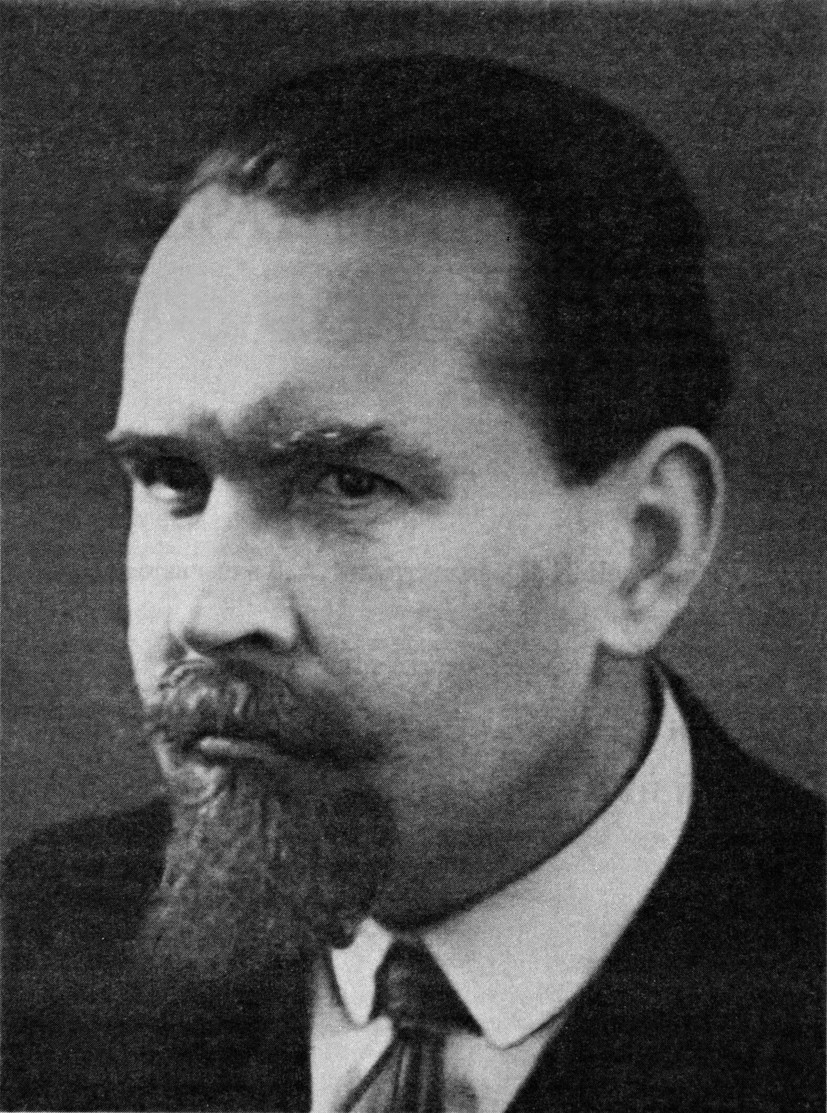
\includegraphics[width=.9\textwidth]{figures/Trubetzkoy.jpg}
  \caption{Prince Nikolai Sergeievič Trubetzkoy}
  \label{fig:ch.prague_trubetzkoy}
\end{wrapfigure}
Of course, {\Trubetzkoy} made no effort to explore these (or other)
distinct consequences of his view of morphophonemic alternations: at
the time he wrote, it was still a major innovation to accord
systematic status to any such notion at all. Indeed, subsequent
discussion of {\Trubetzkoy}'s ideas in the area of \isi{morphophonemics} was
largely critical of his suggestion that there was anything in
particular to account for at all, and his concrete proposals
concerning the nature of morphonemic form were not really taken up by
anyone. Even {\Jakobson}, in works such as his
(\citeyear{jakobson48:russian.conjugation}) article ``{Russian}
Conjugation,'' makes use of a notion of morphophonemic representation
which is much closer to that of {\Bloomfield} (see below,
chapter~\ref{ch.bloomfield}) than to {\Trubetzkoy}'s.

For our purposes, the most important aspect of {\Trubetzkoy}'s view of
the \isi{morphoneme} is the extent to which it is of a piece with the other
constructs of his theory of phonological structure. This theory is
almost exclusively a theory of the \isi{invariant} elements of phonological
\isi{representations}, and accords minimal status to the {rules} which govern
variant realizations of these \isi{representations}. As a result, any
systematic \isi{variation} which is to be incorporated in a description must
be accommodated in the definitions of particular elements. {\Trubetzkoy}
carries this program out in a way which recognizes a range of types of
\isi{variation} in natural language (sub-phonemic phonetic \isi{variation},
\isi{variation} resulting from the \isi{neutralization} of particular \isi{oppositions}
in particular positions, and more general sorts of \isi{alternation}, both
automatic and morphological in nature); but consistent with his basic
position, all of these alternations are treated by appropriate
definition of elements in phonological representation.

Probably no linguist since has attempted to encompass so much of the
sound pattern of natural language entirely within a theory of
\isi{representations} as he did; and a detailed study of the capacities and
limitations of the descriptive framework that he provided would no
doubt cast a good deal of light on the conceptual scope that such a
program is adequate to deal with. Unfortunately, attention in
subsequent years focused largely on the limited area of phonemic form
as delimited by surface \isi{contrast}. Only in the late 1950s and early
1960s did the full range of {\Trubetzkoy}'s concerns reemerge in a
prominent place in phonological theory, bearing by then the clear
impression of the form in which they were passed on to later linguists
by \name{Roman}{Jakobson}.

%%% Local Variables: 
%%% mode: latex
%%% TeX-master: "/Users/sra/Dropbox/Docs/Books/P20C_2/LSP/main.tex"
%%% End: 
